\documentclass[a4paper]{l3proj}
\usepackage{fullpage}
\usepackage{indentfirst}
\usepackage{graphicx}
\usepackage{caption}
\usepackage{subcaption}
\usepackage{enumitem}
\usepackage[usenames,dvipsnames]{xcolor}
\definecolor{customURL}{HTML}{08096E}
\usepackage{hyperref}
\hypersetup{linkcolor=MidnightBlue, urlcolor=customURL, colorlinks}
\usepackage{cite}
\usepackage{minted}

\def\partautorefname{ }
\def\chapterautorefname{\S}
\def\sectionautorefname{\S}
\def\subsectionautorefname{\S}
\def\subsubsectionautorefname{\S}

\setcounter{secnumdepth}{4}
\graphicspath{ {images/} }
\begin{document}
\title{A Social Network for Project Task Management}
\author{Gustavo Almansa\\
      Darren Burns \\
      Leonardo Linhares \\
      Euan Parker \\
	  Tom Wallis \\
}
\date{13 October 2014}
\maketitle
\begin{abstract}

The experimental application presented in this paper explores an alternative approach to project management which allows developers to focus on communication rather than on inputting data into ticket management systems. Since for each ticket there often exists a corresponding conversation, the system tightly integrates instant messaging and ticket management. In doing this, the application is able to emphasise  communication whilst retaining the power of ticket management. Consequently, developers are more likely to make use of the tool since it requires little effort on their part, and managers will remain well-informed as to the progress of the projects they are working on due to an increase in the amount of information available to them.

\end{abstract}
\educationalconsent
\tableofcontents
%============================================================================
\chapter{Introduction}
\label{intro}

%----------------------------------------------------------------------------
\section{Preliminaries}
\label{preliminaries}
A \textit{project management tool} or suite is a program or set of programs which allows a team of developers, managers, and customers to monitor the state of a project. These tools tend to be used to manage tickets. A \textit{ticket} is a collection of items of data used to detail a fault, task or feature.  A \textit{ticket management system} is a type of project management system, whereby it manages and maintains lists of issues documented through tickets. These are notices that members of a development team can set up, discuss code on, and see information about a problem such as its severity and who is responsible for fixing it. Issues and bugs would be found recorded in tickets. They can also hold information about tasks or features that the team has to work on. \textit{Metadata} refers to pieces of data that can be attached to a ticket and contain small pieces of information relating to the topic of discussion. Records of conversations in ticket comment threads help developers to understand the significance of a ticket, and serve as a platform of discussion on active tickets.


%----------------------------------------------------------------------------
\section{Motivation}
\label{motivation}

When writing a software project as a team, it can be difficult to manage issues and bugs. This is generally done in the form of tickets as discussed in the previous section. However, it is often found that programmers discuss these tickets in an informal environment (such as Facebook or Skype) and, once a conversation is had detailing the issue, this work must be carried out a second time in the creation and comments section of a ticket. This is a problem as it duplicates the work that has already been done, wasting time, and the project management tools can be cumbersome to use, making it difficult for users to integrate into their work schedule. Existing management schemes also result in a fragmentation across the different tools being used. Although attempts have been made to make extermal metadata available within conversations, the opposite approach of using the conversations as a source of metadata remain unexplored.

%----------------------------------------------------------------------------
\section{Aims}
\label{aims}

The primary objective of the project is to build a conversation based project management tool.  This tool can then be used to investigate the effectiveness of conversation based tools in managing a project. An additional aim is to investigate how data generated within conversations can be used to simplify ticket management, without compromising on the utility of traditional systems. Because traditional ticket and project management has very little focus on communication, a third aim is to reduce the number of tools a team must employ by providing many functionalities within the one service.

%----------------------------------------------------------------------------
\section{Outline}
\label{outline}

This dissertation will discuss what was achieved during the process of developing the system.

\autoref{research} \textbf{Research} 
This section discusses research that was done on similar products, and what was noted about their design with regards to planning the system.

\autoref{initialPlanning} \textbf{Initial Planning} 
This section discusses how the requirements of the system were developed, and how using this user stories, a user interface mockup and an ER diagram for our system were developed.

\autoref{impl} \textbf{Implementation} 
An overview of the process of implementing the system, detailing the creation of different components of the system such as interface, chat system and model layer, as well as how the project progressed over time.

\autoref{evaluation} \textbf{Evaluation} 
How the project was evaluated.  This will detail the results of the dogfooding, peer evaluation from another team using the system, and improvements to the system that were identified from this feedback.

\autoref{conclusion} \textbf{Conclusion} 
This will detail the current state of the system, whether the aims of the project were achieved, and potential future work that could be done on the system.

%============================================================================

\chapter{Research}
\label{research}

Numerous systems have been developed which aim improve the way in which software projects are managed.

It was found that ticket management systems tend to fall into three categories: ticket centric systems, conversation-based systems, and systems that focused on task management rather than tickets specifically. 

\section{Ticket Centric Systems}

%----------------------------------------------------------------------------
\subsection{Bugzilla}
\label{bugzilla}

Bugzilla \cite{site:bugzilla} is a bug tracker and testing tool created and used by Mozilla. It integrates with several version control systems such as Git and SVN.  Some interesting features include automated reminders, whereby when bugs are reported but left unresolved the system can be configured to send regular emails to specific people informing them of these bugs. This system is known as the ``whine'' system.  When any change is made to a known bug, this change is added to an automated bug report.  Bugzilla integrates with e-mail, whereby these reports can be e-mailed to the user. Although comparatively simple to use, criticisms of Bugzilla have been made that it is hard to manage errors and there exist many bugs in the program itself.

%----------------------------------------------------------------------------
\subsection{Jira}
\label{jira}
JIRA \cite{site:jira1} is a well-used tool for project management, made by Atlassian. Atlassian have a history of working with various aspects of project management, and JIRA integrates with many of these to produce a coherent management environment. However, this makes JIRA less useful on its own, and so there is an identifiable need for a standalone solution, too. Many users of JIRA complain of its difficulty to use, and say that it can be a burdensome way to manage their projects.

\section{Conversation Focused Systems}

%----------------------------------------------------------------------------
\subsection{Slack}
\label{slack}
Slack \cite{site:slack} is an instant messaging system focussed around project management. It can be used in any team-based project, but excels at the management of software projects due to the large number of external services it integrates with, such as GitHub. Despite Slack not providing a mechanism for directly attaching project related issues to conversations, it was decided that the excellent messaging functionality it provides is something that the project should aim to emulate.


\section{Task-Based Systems}
%----------------------------------------------------------------------------
\subsection{Asana}
\label{asana}

The unique selling proposition offered by Asana \cite{site:asana} is effective task management without reliance on email. However, the web interface it offers is difficult to understand, and thus results in a large learning curve. Asana also lacks a real-time communication system, relying on comments on tasks for users to communicate. Whilst analysing this product it was found that relying on commenting rather than instant messaging resulted in a lack of urgency, and users were not as inclined to immediately respond. Consequently, users may choose to rely on an external messaging system for communication.

%----------------------------------------------------------------------------
\subsection{Producteev}
\label{producteev}

Producteev \cite{site:producteev} provides a feature set similar to the aforementioned products, but allows skilled users to quickly navigate the system using numerous shortcuts. A critical feature of Producteev is the ability to convert an email into a task using a Microsoft Outlook extension, thus allowing users to create tasks without have to repeat themselves. 

%----------------------------------------------------------------------------
\subsection{Trello}
\label{trello}

Trello \cite{site:trello} is a web-based task management platform which employs the Japanese ``Kanban''
system, originally developed by Toyota. Kanban uses a hierarchical system of
cards, contained within lists, which themselves are contained within boards, to
manage how projects are managed. Kanban is often used to understand the flow of data within the real world, such as in supermarket production lines or in law cases, but also in project management using Trello.

The team used Trello in the early stages of the project before eventually migrating to use the project itself.

\section{Misc}

%----------------------------------------------------------------------------
\subsection{Codebook}
\label{codebook}
Codebook \cite{site:codebook} was a project management system theorised by Microsoft to visualise the connections between people and their software projects. The project failed to become a public product, but should be noted due to its high degree of social networking and understanding of metadata.

Codebooks most significant lacking in reference to this project’s goals was ticket management. It was not possible to manage a project entirely through Codebook, because it had no ticket management or communication between groups of people; instead, Codebook mapped out projects so workflows could be better understood.

Codebook was never a project that was released to the public, but Microsoft published several papers on it.

%============================================================================
\chapter{Initial Planning}
\label{initialPlanning}
Having researched other products on the market, the team began planning the project itself. 

%----------------------------------------------------------------------------
\section{Team Organisation}
\label{organisation}

In managing the development of the system the team determined a set of tools that would be used.  A means for team members to communicate, store code, divide tasks and document the process was decided upon.

%----------------------------------------------------------------------------
\subsection{Communication}
\label{communication}
Trello \cite{site:ourTrello} was chosen as the team's initial task management software, with the intent to swap to the tool being developed when the project had advanced sufficiently. Facebook chat was used to communicate and arrange meetings.  This split of organisation between Facebook and Trello frustrated some team members which further reinforced the aim of the project - bypassing the repetition of certain tasks over different tools.

%----------------------------------------------------------------------------
\subsection{Version Control}
\label{version}

The team elected to use Git \cite{site:github} as the version control system to manage changes in the source code of the software. Git was used due to multiple team members being familiar with it, and for the integration it has with Github \cite{site:ourGithub}. Making use of version control was vital during development of the project, since features were often being developed simultaneously.


%----------------------------------------------------------------------------
\subsection{Team Roles}
\label{roles}

A set of roles were identified and different team members were provisionally allocated these at the start of the project, as follows.

\begin{itemize}
\item Project Manager: Tom
\item Secretary: Euan
\item Tool Smith: Darren
\item Test Manager: Leo
\item Chief Architect: Gustavo
\end{itemize}

These roles were distributed informally and over time each members duties changed as pertained to their strengths.

%----------------------------------------------------------------------------
\section{Approaching The Problem}
\label{requirements}

The problem that the project aims to solve was established in the initial meetings with the project supervisor. However, developing a set of requirements which would implement a solution for this problem proved more difficult. One of the primary aims of this project is to realise a system which would reduce the duplication of effort that is often required when managing tickets: a team discusses an issue or bug on one platform, and then logs the result in a ticket. This is a problem that existing solutions often make very little or no attempt to solve. Whilst carrying out analysis of existing products and ideas, it was found that Producteev and Codebook attempt to minimise the effects of this issue, and the other systems choose to ignore it completely.

Codebook attempted to solve this problem by closely integrating a social network with software project artifacts. The social network aspect of Codebook was noted by the team as one that may encourage users to use the system both as their primary communication method, and as their project management tool. It was also identified that by giving the software access to tickets and the discussions related to them, a wealth of additional data is available which would otherwise have to be manually entered by a user.

The approach taken by Producteev on the other hand, is to attempt to reduce duplication of effort by allowing users to convert emails into tasks. By allowing users to create a task in this way, the need to copy information from email to the task manually is overcome.

Both of these features helped inspire the primary requirements of the software. It was deemed a vital requirement that the software tightly integrate social features in order to make use of the data generated through users communicating with each other. In addition, the team decided that the software needed to use this data in order to minimise the effort required in managing a software project. Agile software development aims to prioritise interactions over process, and so it would be prudent to design the software to maintain some degree of process without overly interfering with communication.

It was noted that the products that were looked at often had native apps and websites designed for desktop, but very few employed a responsive design to cater to their mobile users. It was decided that the design of the project must provide for the variety of devices the user may use to navigate the site, and that the website should accommodate for all possible cases.

Several different ideas for the development of the system were discussed. One suggested approach was that an existing product be extended to attempt to meet the requirements. Suggestions for implementing this approach included:

\begin{itemize}
\item \textit{Interfacing a custom ticket management system with Skype}. \par This approach was rejected due to the lack of control that the Skype API gives with regards to accessing data contained within conversations.
\item \textit{Creating an instant messaging extension for Jira}. \par This approach was rejected due to the emphasis that Jira places on the ticket based approach. Although the required design would have to maintain aspects of this approach, it would have been difficult to focus on communication when there is a major dependence on a colossal, process reliant ticket management system.
\item \textit{Use the Facebook API as a basis for a chat system}. \par  It was found that the Facebook API for integrating with the chat system is extremely limited and therefore would not have been suitable for achieving the requirements of this project.

\end{itemize}

With none of these approaches offering the desired flexibility, it was decided to build the system using Django, a Python web development framework. Django has a thriving developer community and its popularity means that it is easy to find tutorials and answers to questions should problems arise. It is also exceptionally powerful when it comes to interfacing with database management systems, providing an easy to use interface allowing Python code to treat database records as Python objects by defining mapping classes known as “models”. As a result of this decision, and in addition to the extensive research of existing project management systems, an initial set of user stories were developed.

%----------------------------------------------------------------------------
\section{User Stories}
\label{userStories}

Listed below is the collection of user stories that were initially created for the system.  Over time these were added to, modified and removed depending on various decisions regarding development of the system.

\begin{enumerate}[ref=\arabic*]
\item As a \textit{user} I want to \textit{create an account} on the system so that I can \textit{use the features it offers}. \label{item:1}
\item As a \textit{user} I want to \textit{create a conversation with another user} so that I can \textit{discuss a proposed change}. \label{item:2}
\item As a \textit{project manager} I want to \textit{change other users privileges} so that \textit{I limit other users access}. \label{item:3}
\item  a \textit{developer} I want to \textit{tag a conversation as a ticket} so that \textit{it becomes managed}.\label{item:4}
\item As a \textit{developer} I want to \textit{attach additional meta-data to a ticket} to allow me to keep track of priority, progress and other issues.\label{item:5}
\item As a \textit{developer} I want to \textit{end a conversation or ticket} so that I\textit{don't have to look at irrelevant tickets}.\label{item6}
\item As a \textit{developer} I want to \textit{be able to change priorities of my tickets} so that \textit{more important tasks get priority}.\label{item:7}
\item As a \textit{QA manager} I want to \textit{be able to change the priorities of other peoples tickets} so that I can \textit{decide the importance of certain tasks}.\label{item:8}
\item As a \textit{developer} I want to \textit{assign milestones to a conversation} so that I can \textit{track project velocity}.\label{item:9}
\item As a \textit{developer} I want to \textit{split a conversation} so that I can \textit{separate multiple issues if they appear in a single ticket}.\label{item:10}
\item As a \textit{user} I want to \textit{tag another user} to \textit{add them to a discussion}.\label{item:11}
\item As a \textit{project manager} I want to \textit{view metrics that have been extracted from a ticket} so that I can \textit{monitor my teams progress on an issue}.\label{item:12}
\item As a \textit{developer} I want to \textit{link to a version control repository} so that I can \textit{quickly access the technical side of the ticket}.\label{item:13}
\item As a \textit{user} I want to \textit{attach multimedia to a conversation or ticket} so that I can \textit{explain problems or ideas more easily}.\label{item:14}
\item As a \textit{developer} I want to \textit{assign resolution to an owner} so that it will get done.\label{item:15}
\item As a \textit{user} I want to \textit{add other people to help resolve the issue}.\label{item:16}
\item As a \textit{user} I want to \textit{be able to autocomplete names of other users} so that I can \textit{tag other users correctly and quickly}.\label{item:17}
\item As a \textit{user} I want to \textit{create labels} so that I can \textit{cross reference other conversations}.\label{item:18}
\item As a \textit{developer} I want to \textit{view previous tickets} so that I can \textit{view what has been changed previously}.\label{item:19}
\item As a \textit{project manager} I want to \textit{track the activity of other users} so that I \textit{know what is happening in the project}.\label{item:20}
\item As a \textit{user} I want to \textit{search the website} so that I can \textit{find things within the site quickly}.\label{item:21}
\end{enumerate}

From these user stories a set of high, medium and low priority tasks were determined. The high priority user stories were: \ref{item:1}, \ref{item:2}, \ref{item:5}, \ref{item:7}, \ref{item:12}, \ref{item:19}. Medium priority: \ref{item:11}, \ref{item:15}, \ref{item:18}. Low priority: \ref{item:10}, \ref{item:13}, \ref{item:14}, \ref{item:17}.

\iffalse
\subsection{High Priority}
\begin{itemize}
\item \textit{Create an account} \par
The first page a user should see when loading the website must be a page asking them to log in, or create a new account if they have not already done so.
\item \textit{Create a conversation} \par
There must be a way to create a new conversation to discuss different topics relating to the project.
\item \textit{Create a project} \par
There must be a way to create a new project to manage within the software. 
\item \textit{Add metadata to a conversation} \par
Users must be able to attach relevant metadata to conversations.  Attaching additional information to a chat system is crucial in achieving the goal of combining a ticketing system with social networking.
\item \textit{Change priority of conversations} \par
A user must be able to change the priority of a conversation so that high priority tasks get more attention.  This goes hand-in-hand with adding metadata, whereby priority could be represented as a metadata object.
\item \textit{View previous closed conversations} \par
Viewing previous conversations is essential in seeing what has been achieved so far over the course of a project's lifespan.
\item \textit{View visualisations based on data extracted from conversations} \par
Viewing visual representations of different aspects of a project allows users to determine how much effort is being devoted to a project, how many people are working on a project and each users individual contribution.
\end{itemize}
\subsection{Medium Priority}
\begin{itemize}
\item \textit{Assign resolution of a conversation to an owner} \par
Users should be able to assign a conversation to another user in order to regulate who works on what issue.  This prevents multiple people working on the same thing while another task goes undone.
\item \textit{Tagging other users in a conversation to bring it to their attention} \par
Users should be able to tag other users in a conversation, so that when the subject being discussed relates to.
\item \textit{Linking to other conversations to cross reference discussions} \par
In the event that multiple conversations have a common topic there should be a way to link these conversations, as this allows users to quickly find relevant information pertaining to the topic.
\item \textit{Filtering conversations} \par
Users should be able to filter conversations by typing text for which to search for, and remove any conversations that do not contain these terms.
\item \textit{Saving messages within chats} \par
Users should be able to save messages within chats, so that messages that contain important messages or links can be quickly found.

\end{itemize}
\subsection{Low Priority}
\begin{itemize}
\item \textit{Linking to version control repository} \par
Users could be able to link to version control, so that it is quicker for teams to navigate between different tools relating to the management of the project.

\item \textit{Attach multimedia to a conversation} \par
Attaching media to a conversation could be useful as users may wish to link videos, images or sound clips containing relevant information.

\item \textit{Autocomplete names of users} \par
Autocompleting user names can make it easier to tag other users by ensuring their name is correctly typed.

\item \textit{Branching conversations to separate different issues} \par
Branching conversations could be useful as it allows a discussion that involves multiple topics to be split up into separate conversations, allowing users to only read through information that is relevant.

\end{itemize}

\fi


%----------------------------------------------------------------------------
\section{Design}
\label{design}

Once the initial requirements were established an entity-relationship (ER) diagram was developed. After several iterations, the diagram shown in \autoref{figure:ERDiagram1} was produced. This was used to assist the development by identifying the crucial components of the system. Additionally, the ER diagram greatly aided in the modelling of the data using the Django Object Relational Mapper, since there is a close correlation between the features of the diagram and the structure of data models in Django.

Due to the experimental nature of the project, rapidly changing requirements meant that that the final model of the system varies from the design in the diagram.

Next, a series of paper based prototypes were created in order to plan the user interface. Paper prototyping was used due to the quick, easy and inexpensive nature whereby multiple different possible designs can be quickly produced and contrasted. Several initial designs were brainstormed. The clutter, intuitiveness and overall appeal of different designs were compared.  Examples of different designs that were considered are shown below.

\begin{figure}
\centering
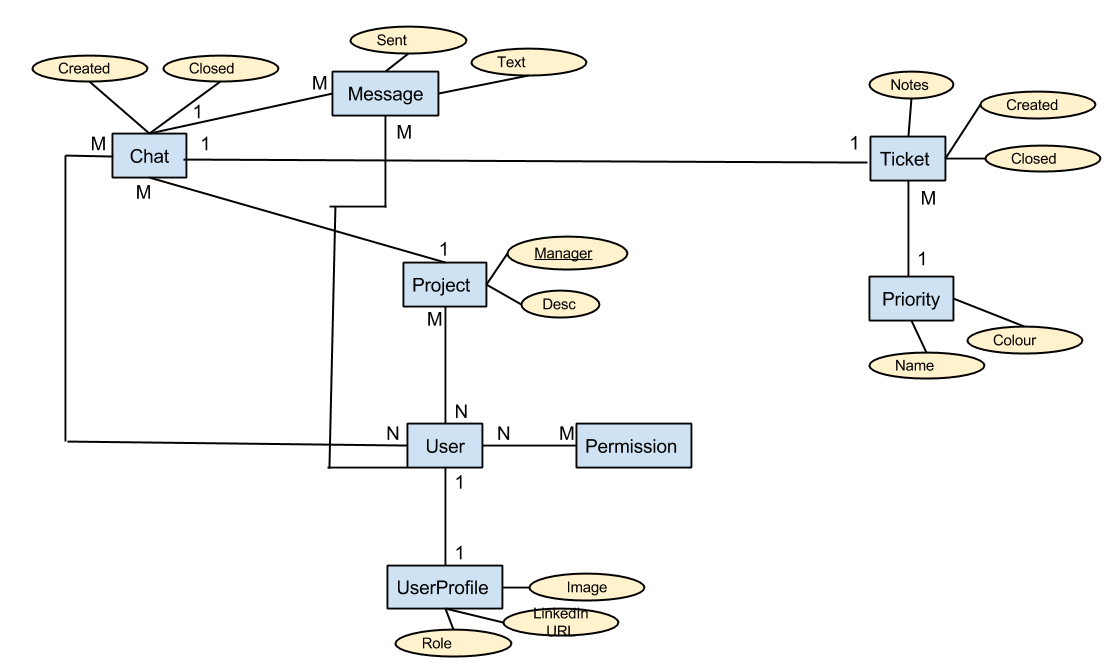
\includegraphics[scale=0.4]{ER_Diagram}
\caption{ER Diagram}
\label{figure:ERDiagram1}
\end{figure} 

\begin{figure}
    \centering
    \begin{subfigure}[b]{0.3\textwidth}
	    \centering
		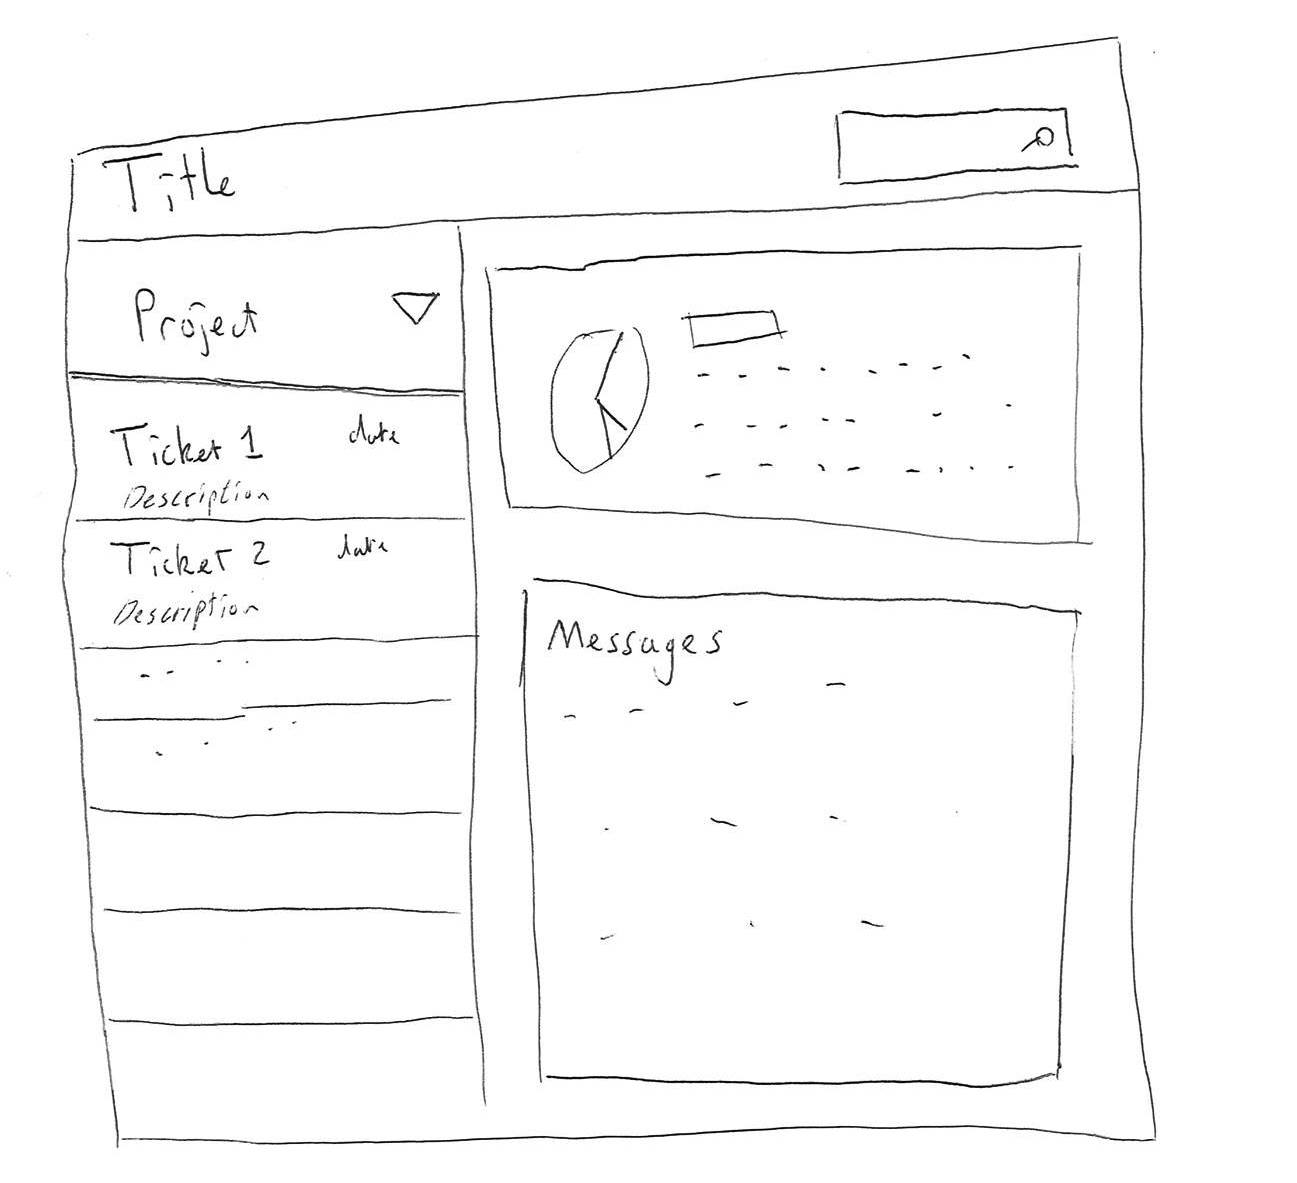
\includegraphics[width=\textwidth]{mockup1}
		\caption{Mockup 1}
		\label{fig:mockup1}        
    \end{subfigure}
    \hfill
    \begin{subfigure}[b]{0.3\textwidth}
        \centering
		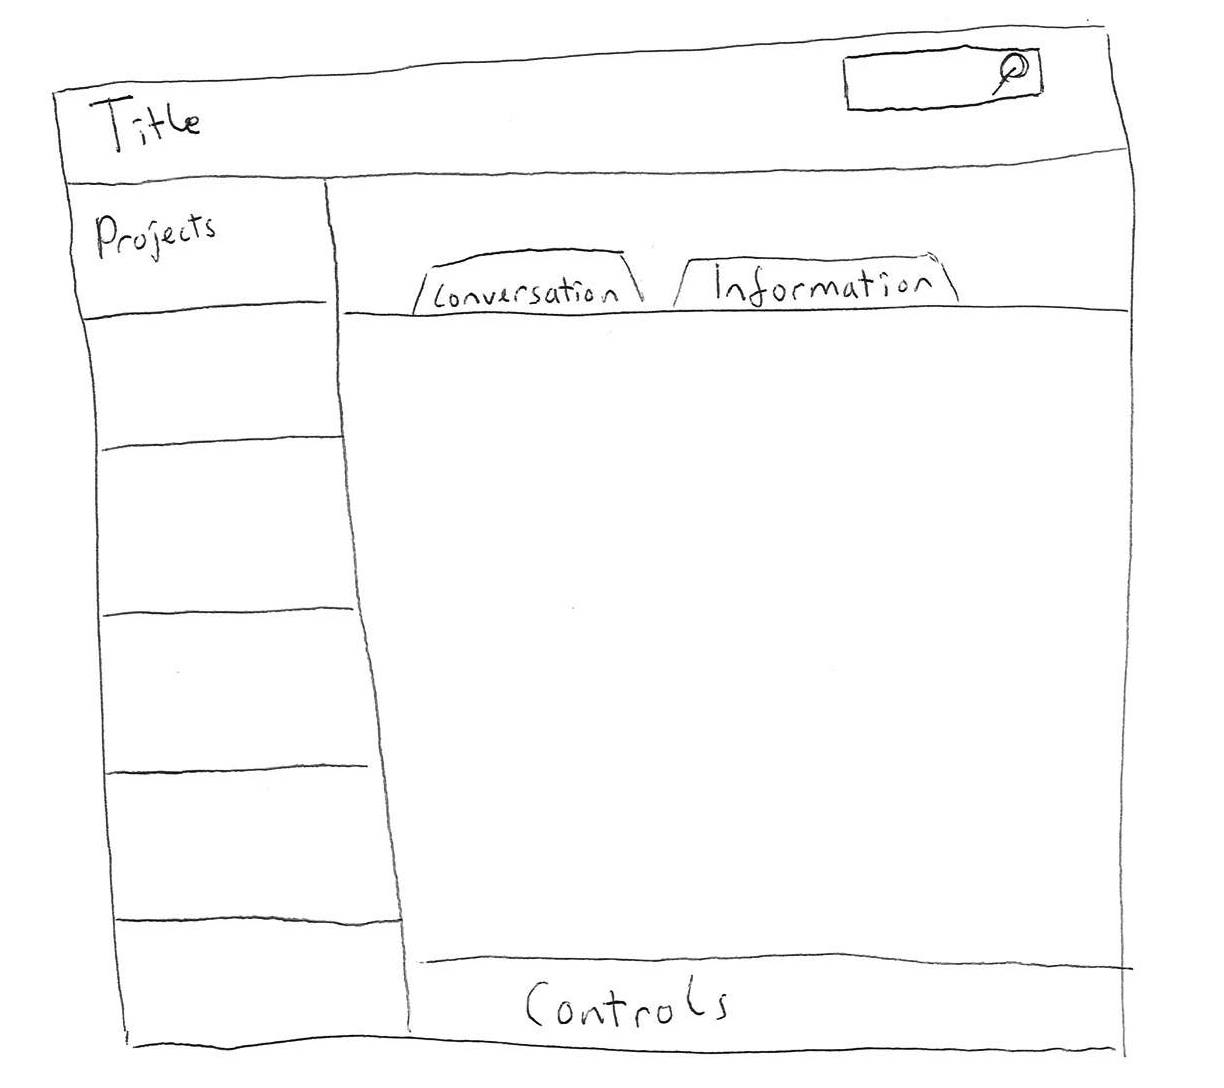
\includegraphics[width=\textwidth]{mockup2}
		\caption{Mockup 2}
		\label{fig:mockup2} 
    \end{subfigure}
    \hfill
    \begin{subfigure}[b]{0.3\textwidth}
        \centering
		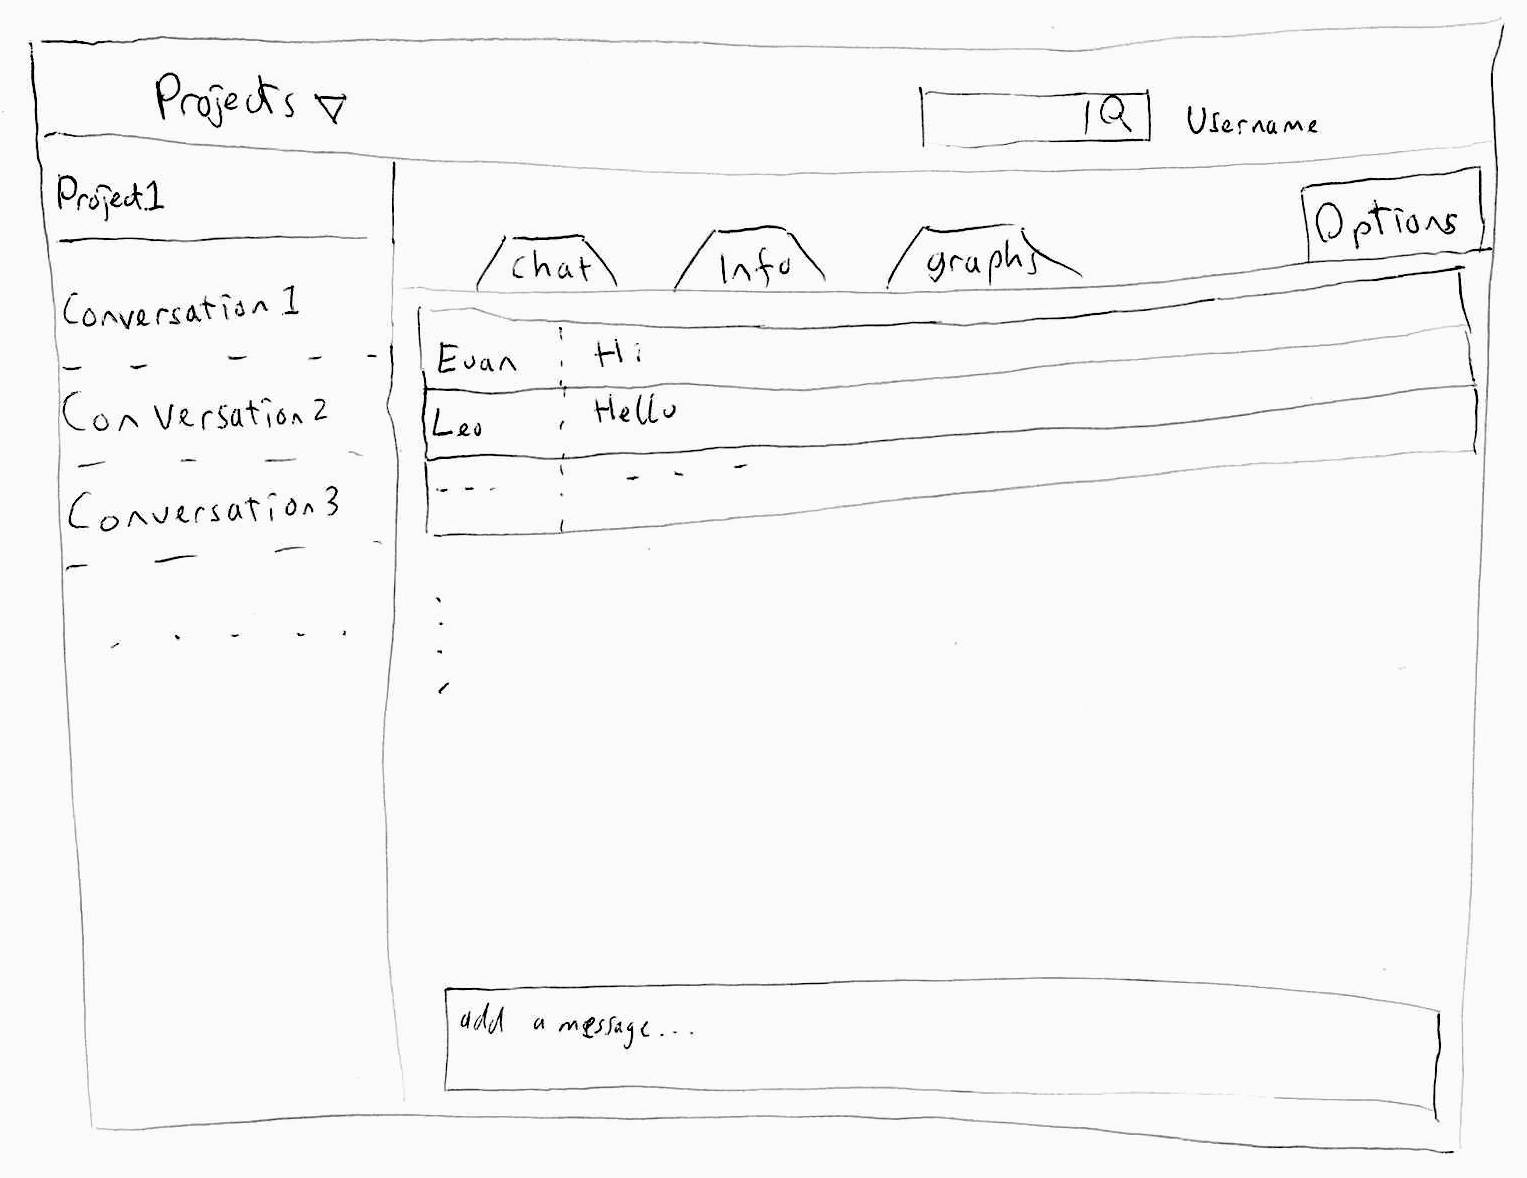
\includegraphics[width=\textwidth]{mockup3}
		\caption{Mockup 3}
		\label{fig:mockup3} 
    \end{subfigure}
    \caption{Three mockups}
    \label{fig:Three mockups}
\end{figure}

\autoref{fig:mockup1} shows the initial prototype for the design, which displayed visualisations relating to the project on the main page.  A project was chosen from a dropdown menu and all the tickets related to that project were listed below.   Each ticket consisted of the graphs, metadata and the associated conversation.

In \autoref{fig:mockup2}, the ticket appearance was changed whereby the information section was removed and two tabs were added, a ‘conversation’ tab which was used to display the messages, and an ‘information’ tab which displayed visualisations and metadata related to the project. This change was made to reduce clutter in the interface and  A controls section was added which would be used to add new metadata such as due date, priority, assignee etc.

The final design, \autoref{fig:mockup3}, moved the projects drop-down menu into the navbar, with the selected project shown below alongside the relevant conversations.  The controls section was removed and an options menu was added above the conversations.  The information tab was divided into an info and graphs tab, whereby info contained metadata relating to the conversation and graphs contained the visualisations that had been generated with the data.




%============================================================================
\chapter{Implementation}
\label{impl}

Once the requirements had been identified and the way the team was to organise itself had been formalised implementation could begin. 

The server side of the application is written in Python, using the Django web application framework and several additional Python modules. A second server exists purely for handling real time communications. The client side is written using the jQuery Javascript library \cite{site:jquery}, with several other Javascript libraries being used to handle different components such as chat and graphs. 

%----------------------------------------------------------------------------
\section{Workflow}
\label{workflow}

%----------------------------------------------------------------------------
\subsection{Git}
\label{git}

Several branches were maintained within the Git repository. Two of these branches were particularly important, as they represented primary and secondary deployments of the project. The master branch contained the most stable build, and the beta branch was used as a deployment staging area for new features. Some code modifications may work as intended in a development environment and then break when deployed. To overcome this risk, code was first deployed to the beta branch before being merged into the master branch.

One aspect of version control in which the team was eventually diligent in applying was continuous integration, in which feature branches are regularly merged into the master branch. Using continuous integration meant that the live version of the project never strayed too far from the overall set of features that were being developed at a given time. Frequent merging of feature branches also provided the added benefit that breaking changes were easier to find, due to the fact that less code was being added in each merge. During the initial stages of the project, branches often went unmerged for several weeks, making integration of features exceptionally difficult. After realising the difficulties this workflow caused, this flaw was amended by substantially increasing the rate at which features were merged with the master branch. Diagram \ref{figure:diagram1} shows how features were frequently merged into the master branch (shown as the black line at the top of the diagram) during the week of March 1st 2015.

\begin{figure}[ht, ref={\alph}]
\centering
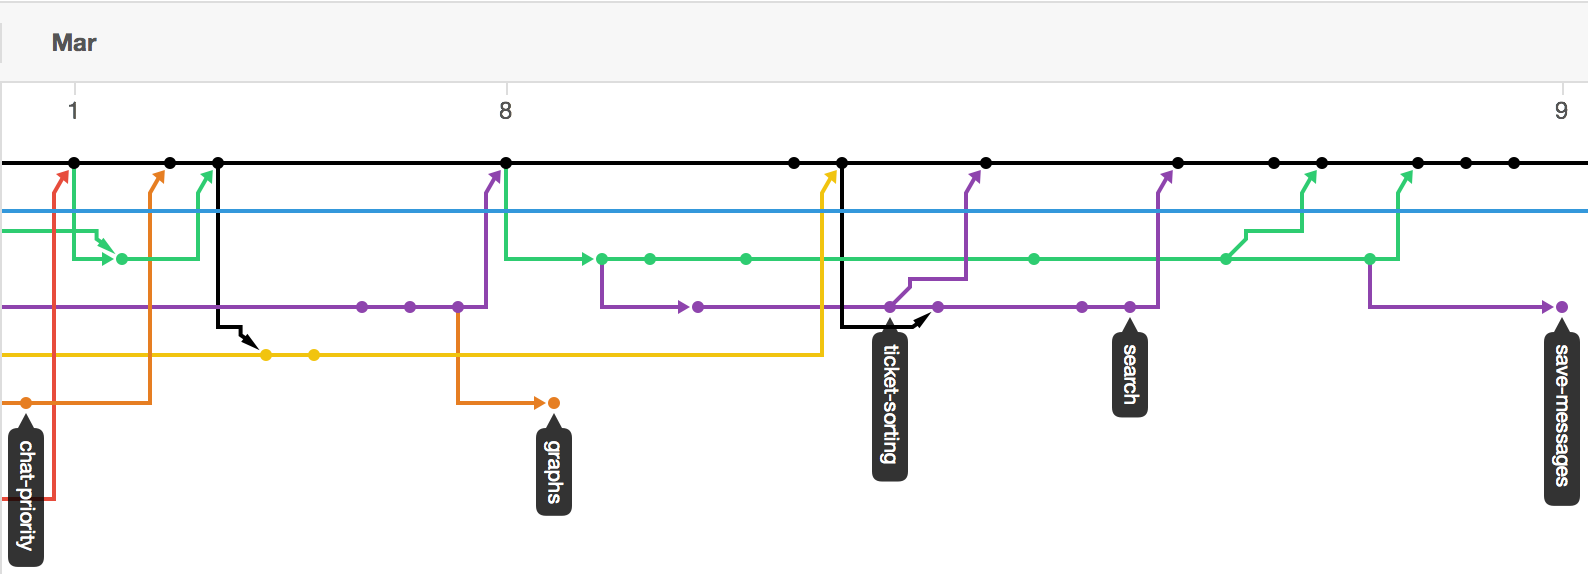
\includegraphics[scale=0.5]{diagram}
\caption{Branching Diagram 1}
\label{figure:diagram1}
\end{figure} 

\begin{figure}[ht, ref={\alph}]
\centering
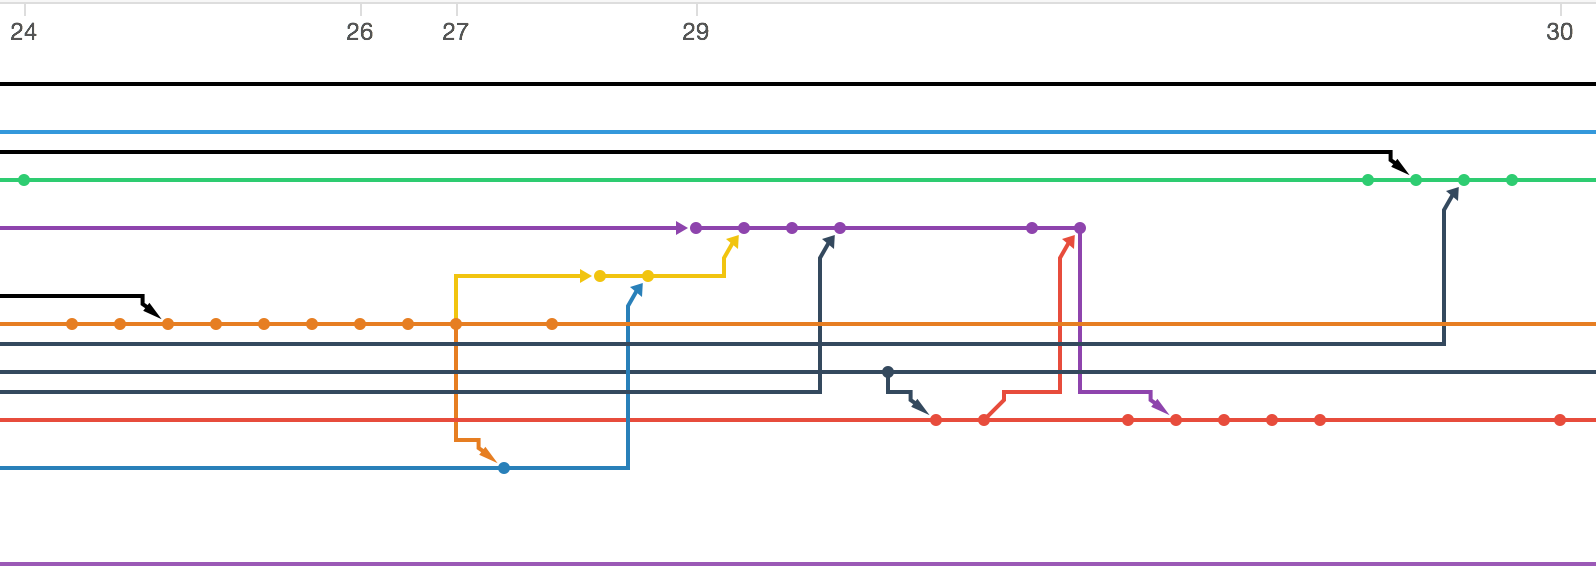
\includegraphics[scale=0.5]{diagram2}
\caption{Branching Diagram 2}
\label{figure:diagram2}
\end{figure} 

For comparison, the lack of feature branch integration exhibited during the early stages of the project is displayed in diagram \ref{figure:diagram2}, which shows branching activity between the 24th and 30th of November 2014.

%----------------------------------------------------------------------------
\subsection{Continuous Delivery}
\label{continuousDelivery}

A service called Codeship was used to ease the deployment of new builds. Codeship \cite{site:codeship} is a continuous deployment platform which was configured so that any changes to the master branch or the beta branch of the Github repository were automatically built and deployed to their respective live websites.

%----------------------------------------------------------------------------
\section{Deployment}
\label{deployment}

An unforeseen benefit of using the combination of Git and Github was the ease by which the system could be deployed. Two instances of the project \cite{site:liveproject} were hosted on Heroku \cite{site:heroku}, a platform for hosting dynamically scalable web applications. The first instance hosted the code held within the master branch of the Git repository. The second instance ran the code present in the “beta” branch of the project. Heroku provides a mechanism which enables deployment using Git, so the deployed version of the product is always equivalent to the most recent commit on the master branch.

Since the default web server provided by Django is not suitable for production use, the Gunicorn \cite{site:gunicorn} server was used instead. Heroku made it easy to use Gunicorn through the use of a “Procfile”, which specifies the Bash commands that should be executed whenever a write is made to the master branch of the repository. Thus, using Gunicorn was as simple as adding the initialisation command to this file.

A Python library known as WhiteNoise \cite{site:whitenoise} was used to index static assets, such as images, Javascript, and CSS files. Since these assets are indexed into a dictionary, the server can perform an O(1) lookup to retrieve a file requested by the client instead of an O(n) file system traversal resulting in a performance increase.

%----------------------------------------------------------------------------
\section{Model Implementation}
\label{modelImpl}


The data model was implemented as shown in \autoref{figure:ERDiagram} using Django’s built in Object Relational Mapper (ORM). During the initial stages of development, these models were mapped to a SQLite \cite{site:sqlite} schema, but as development progressed, the PostgreSQL database management system was used instead. PostgreSQL \cite{site:postgresql} was used due to the ease by which it can be connected to a Heroku hosted application, whilst SQLite is only suitable for desktop or mobile applications. An additional factor contributing to this decision is that SQLite does not scale well on web applications due to the fact that concurrent access rates can change unpredictably, and are often much higher in comparison to client side applications.


\begin{figure}[ht]
\centering
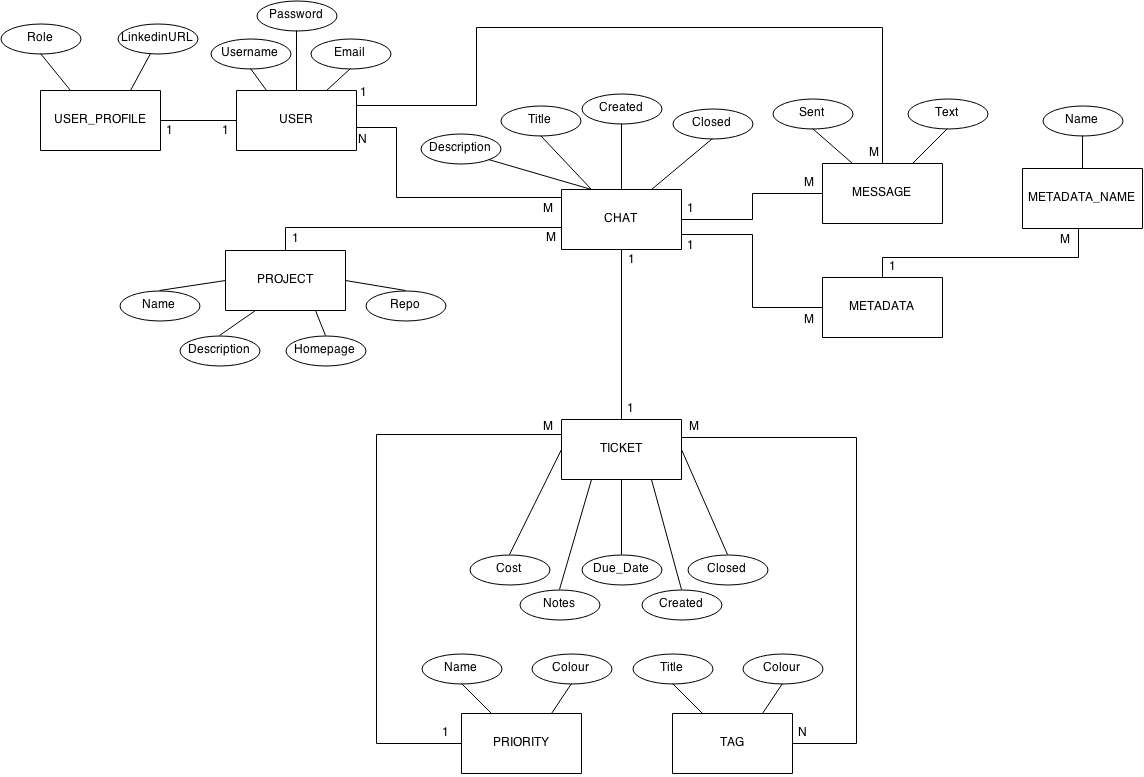
\includegraphics[scale=0.35]{newERdiagram}
\caption{Final ER Diagram}
\label{figure:ERDiagram}
\end{figure}
%----------------------------------------------------------------------------
\section{User Interface}
\label{userInterface}

Due to the system being a web application, the main technologies used in the creation of the user interface were HTML5 and CSS3, as is standard in the vast majority of web based software. 

Twitter’s Bootstrap library was used to manage the layout of web pages, and to improve compatibility with mobile devices. The intuitive grid layout system provided by this library greatly improved the rate at which the UI was developed, since it minimised the extent to which the team had to rely on custom CSS rules.

Bootstrap satisfied the requirement of responsive design due to its feature of being mobile-first when necessary. This meant that the design of the web pages could be laid out in such a way as to accommodate small screens, and expand to larger sizes of screens when necessary.

Certain decisions were made to enhance the user friendliness and quality of user experience during the design of the user interface. When appropriate, the team followed design patterns in line with the German Bauhaus movement of design. Bauhaus design revolves around the idea that the form of a design should be directly influenced by the function of a project. In this case, the function of the application is to allow ticket management with a focus on communication and conversation; therefore, design decisions were made which would ingrain this functionality into the user interface. A tabbed design allowed for immediate access to conversations while allowing access to metadata and metrics. Furthermore, tabbed designs are very common, so this was also easy to use. 
Another example of the design’s form following its function is that the conversations are almost always available via Bootstrap accordions in a sidebar. This allows for easy and constant access to conversations, as a user’s focus, but does not clutter the user’s view at any time due to accordion’s collapsibility and Bootstrap’s minimalist look.

It was identified that the application must be reactive to user interaction, and to accommodate this, the jQuery Javascript library was used. jQuery assists almost every element of the application, from displaying new messages on the screen, to highlighting selected issues. 

Perhaps the most important feature of the jQuery library used to make the website more responsive was Ajax (Asynchronous Javascript and XML). Ajax provides the ability to reload only small portions of the page when required, rather than reloading the entire page and sending multiple requests for objects that have already been transferred. Ajax is the basis for several features of the application that would otherwise respond slowly, such as the search and sort features. It was deemed that a constantly reloading page would be frustrating to a user, particularly a mobile user with potentially slow internet connections. Ajax was an appropriate way of circumventing this problem in a way that would be aesthetically pleasing to the user. 

The resulting design of the project, shown in \autoref{figure:finalproduct}, was a set of pages that were responsive to user input and intuitive to use, which focused on the functionality of the application. In addition, the pages were mobile-ready, meaning that the intuitive design could be shared across any platform. 

\begin{figure}[ht]
\centering
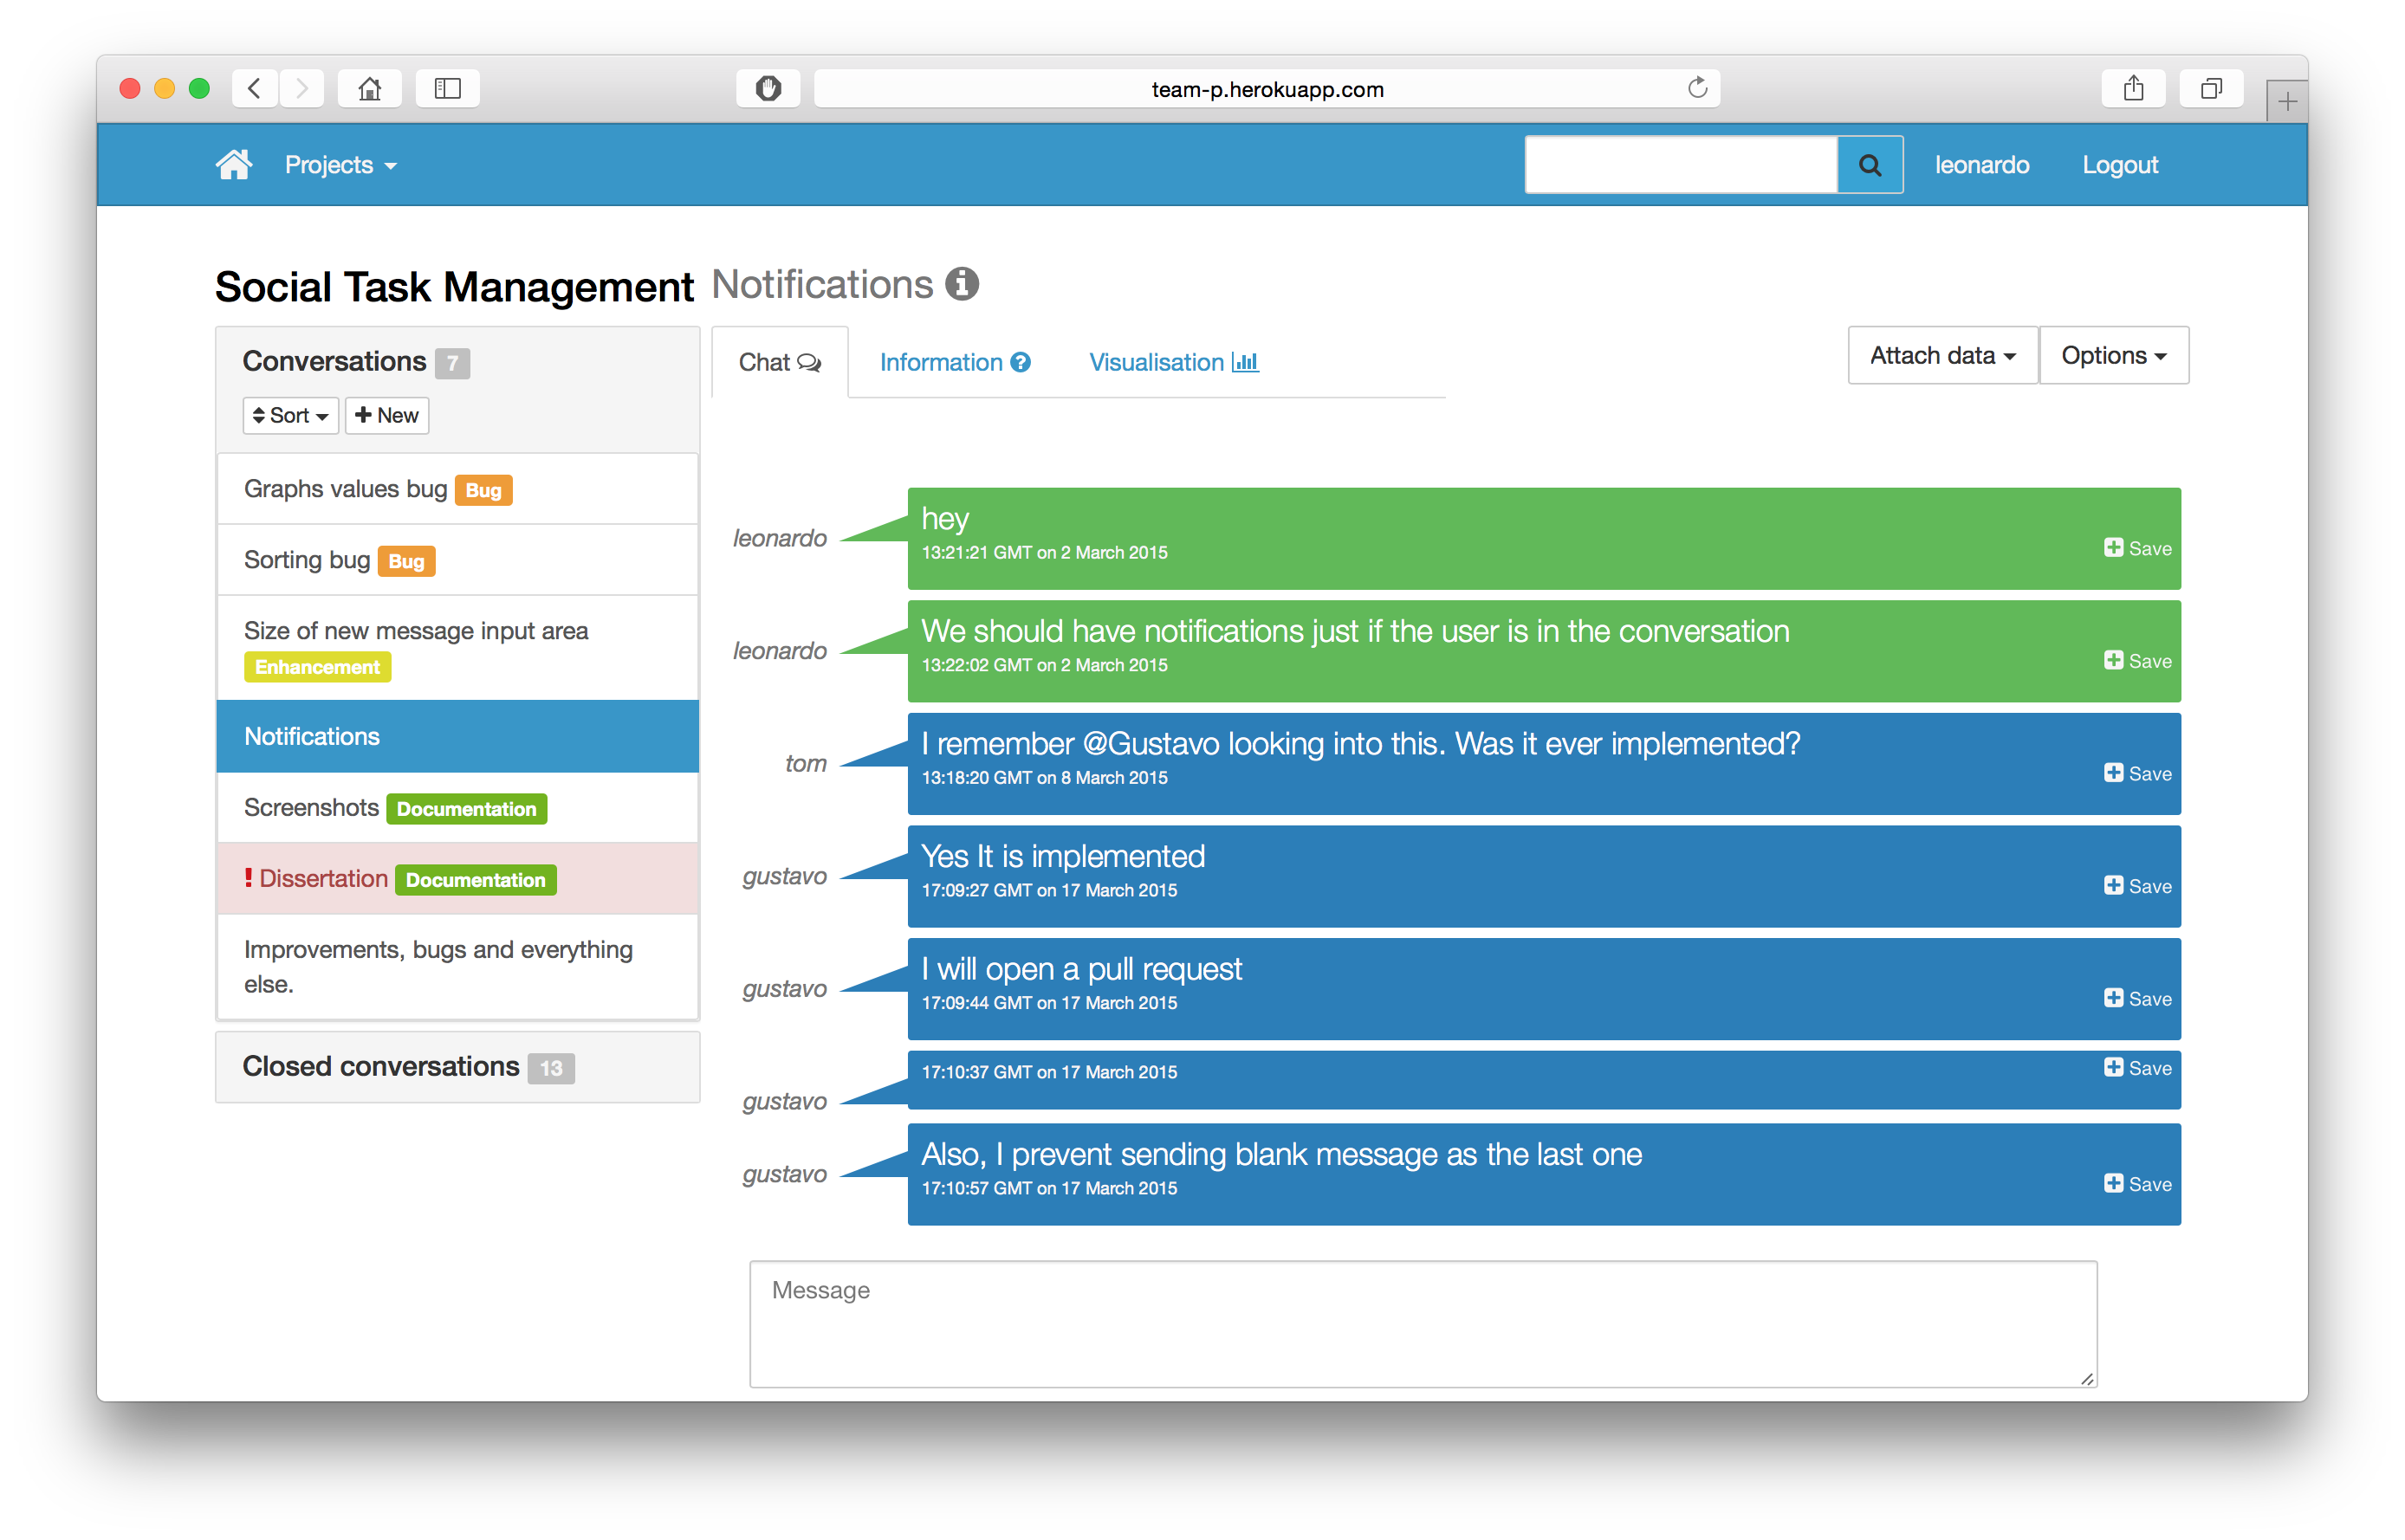
\includegraphics[scale=0.35]{finalproduct}
\caption{Final Design}
\label{figure:finalproduct}
\end{figure}

%----------------------------------------------------------------------------
\section{Messaging System}
\label{messagingSystem}

The instant messaging aspect of the project was implemented using a Javascript library and backend data storage service called Firebase \cite{site:firebase}. An alternative option considered by the team was to implement a server side mechanism for handling messaging using the WebSocket \cite{site:websockets} protocol. However, several disadvantages to this approach were found on investigation:

\begin{itemize}
\item The default Django web server relies on the Web Server Gateway Interface (WSGI) \cite{site:python-webserver} for handling communication between the server and the framework. Due to the request handling mechanism employed by WSGI, it is not possible to support long term connections through the likes of WebSockets, and so an additional server which provides support for the WebSocket protocol would have to be set up to achieve the required functionality.
\item The WebSocket protocol is extremely complex in comparison to the Firebase library, and so it would have been difficult to produce a working system within the time constraints of the project.
\end{itemize}

Another option which was considered was working within the constraints of the Django framework. Creating an instant messaging system within Django would require using an inefficient method such as asynchronous polling, in which the client repeatedly asks the server if a new message has been sent.

The decision to use Firebase was not without its drawbacks:
\begin{itemize}
\item There is an overhead in ensuring that the data in the external storage provided by Firebase remains consistent with the data held within the relational database.
\item Employing a third party storage service added an additional point of failure. On several occasions throughout development, the Firebase API became unavailable, leaving the application unusable for a short period of time
\item Each member of the team had to understand the API exported by Firebase. Consequently, the project uses two REST APIs for communication with the server side rather than one, increasing the complexity of the design. The Firebase API also proved difficult to work at times, with simple queries departing from the widely understood semantics of SQL.
\item The free access to Firebase seemed to randomly throttle connection to its servers, occasionally resulting in slow resolution of API calls.
\end{itemize}

In general, the use of an external service to implement the messaging system greatly improved the rate of development of the project and allowed the team to focus on other aspects of the system, which may not have been possible using one of the other options.

Due to the fact that some messages may try to convey a lot of information, it was felt that the messaging system should allow some level of formatting, enabling users to write formatted lists, headings, emphasised text and more. This was achieved using a Javascript library known as Showdown.js \cite{site:showdown}, which enables users to write messages using the Markdown \cite{site:markdown} formatting language. Before messages are displayed on screen, they are passed through the Markdown parser provided by Showdown.js and converted to valid HTML. \autoref{figure:markdown} shows how Markdown formatted text can improve the readability of what would otherwise be a comma separated list.

\begin{figure}[ht]
\centering
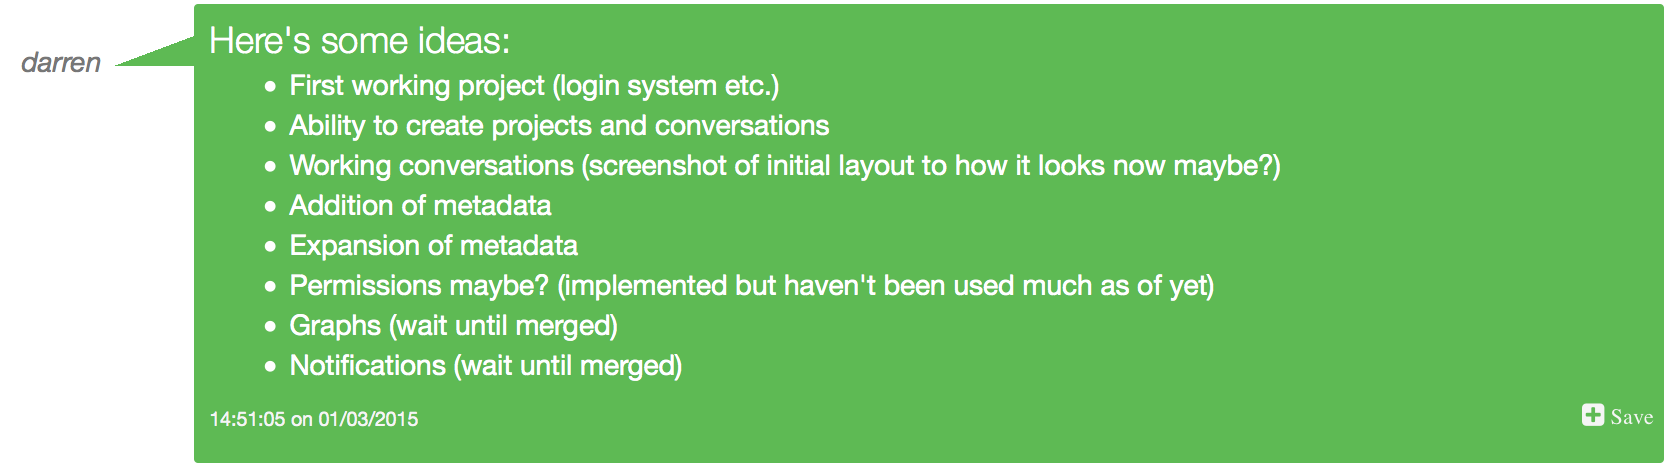
\includegraphics[scale=0.5]{markdownExample}
\caption{Markdown Example - Unordered List}
\label{figure:markdown}
\end{figure}

%----------------------------------------------------------------------------
\section{REST API}
\label{restApi}


A REST API provides an interface between the client and the server. A Django plugin known as TastyPie \cite{site:tastypie} was used to convert the models that were previously defined into REST endpoints that the client can call to request data from the database. After quick initial configuration of the plugin, specified portions of the database schema were available to the client side of the application. For example, if the browser requests the URL \texttt{/api/v1/chat/}, the server will respond with a Javascript Object Notation (JSON) object containing information about all conversations in the database. A truncated typical response from accessing this endpoint is shown below.

\begin{minted}{json}
{
   "meta":{
      "limit":20,
      "next":"/api/v1/chat/?limit=20&offset=20",
      "offset":0,
      "previous":null,
      "total_count":21
   },
   "objects":[
      {
         "closed":"2015-02-15T14:42:08.777264",
         "created":"2015-02-15T14:39:11.757739",
         "description":"",
         "id":5,
         "project":"/api/v1/project/1/",
         "resource_uri":"/api/v1/chat/5/",
         "ticket":{
            "closed":null,
            "cost":null,
            "created":"2015-02-15T14:39:11.795494",
            "due_date":null,
            "id":5,
            "notes":"Done via. migrations",
            "priority":null,
            "resource_uri":"/api/v1/ticket/5/",
            "tag":[],
            "user":null
         }
...
}
\end{minted}

This JSON object can then be parsed using Javascript and injected into the Document Object Model (the tree representing the layout of the document) using Ajax, therefore making it visible to the user without requiring a page refresh.

The system relies heavily on client side processing of data, and so having a flexible and extensive REST API was an essential component of the application, enabling client and server to communicate.
%----------------------------------------------------------------------------
\section{Prototype}
\label{prototype}


A prototype was prepared for demonstration after an initial ten weeks of development. The interface shown in \autoref{figure:prototype} is simple but fully functional. The system had basic functionalities such as: 

\begin{itemize}
\item User registration and login
\item Project creation
\item Creation of independent conversations
\item Closing of conversations
\end{itemize}

\begin{figure}[ht]
\centering
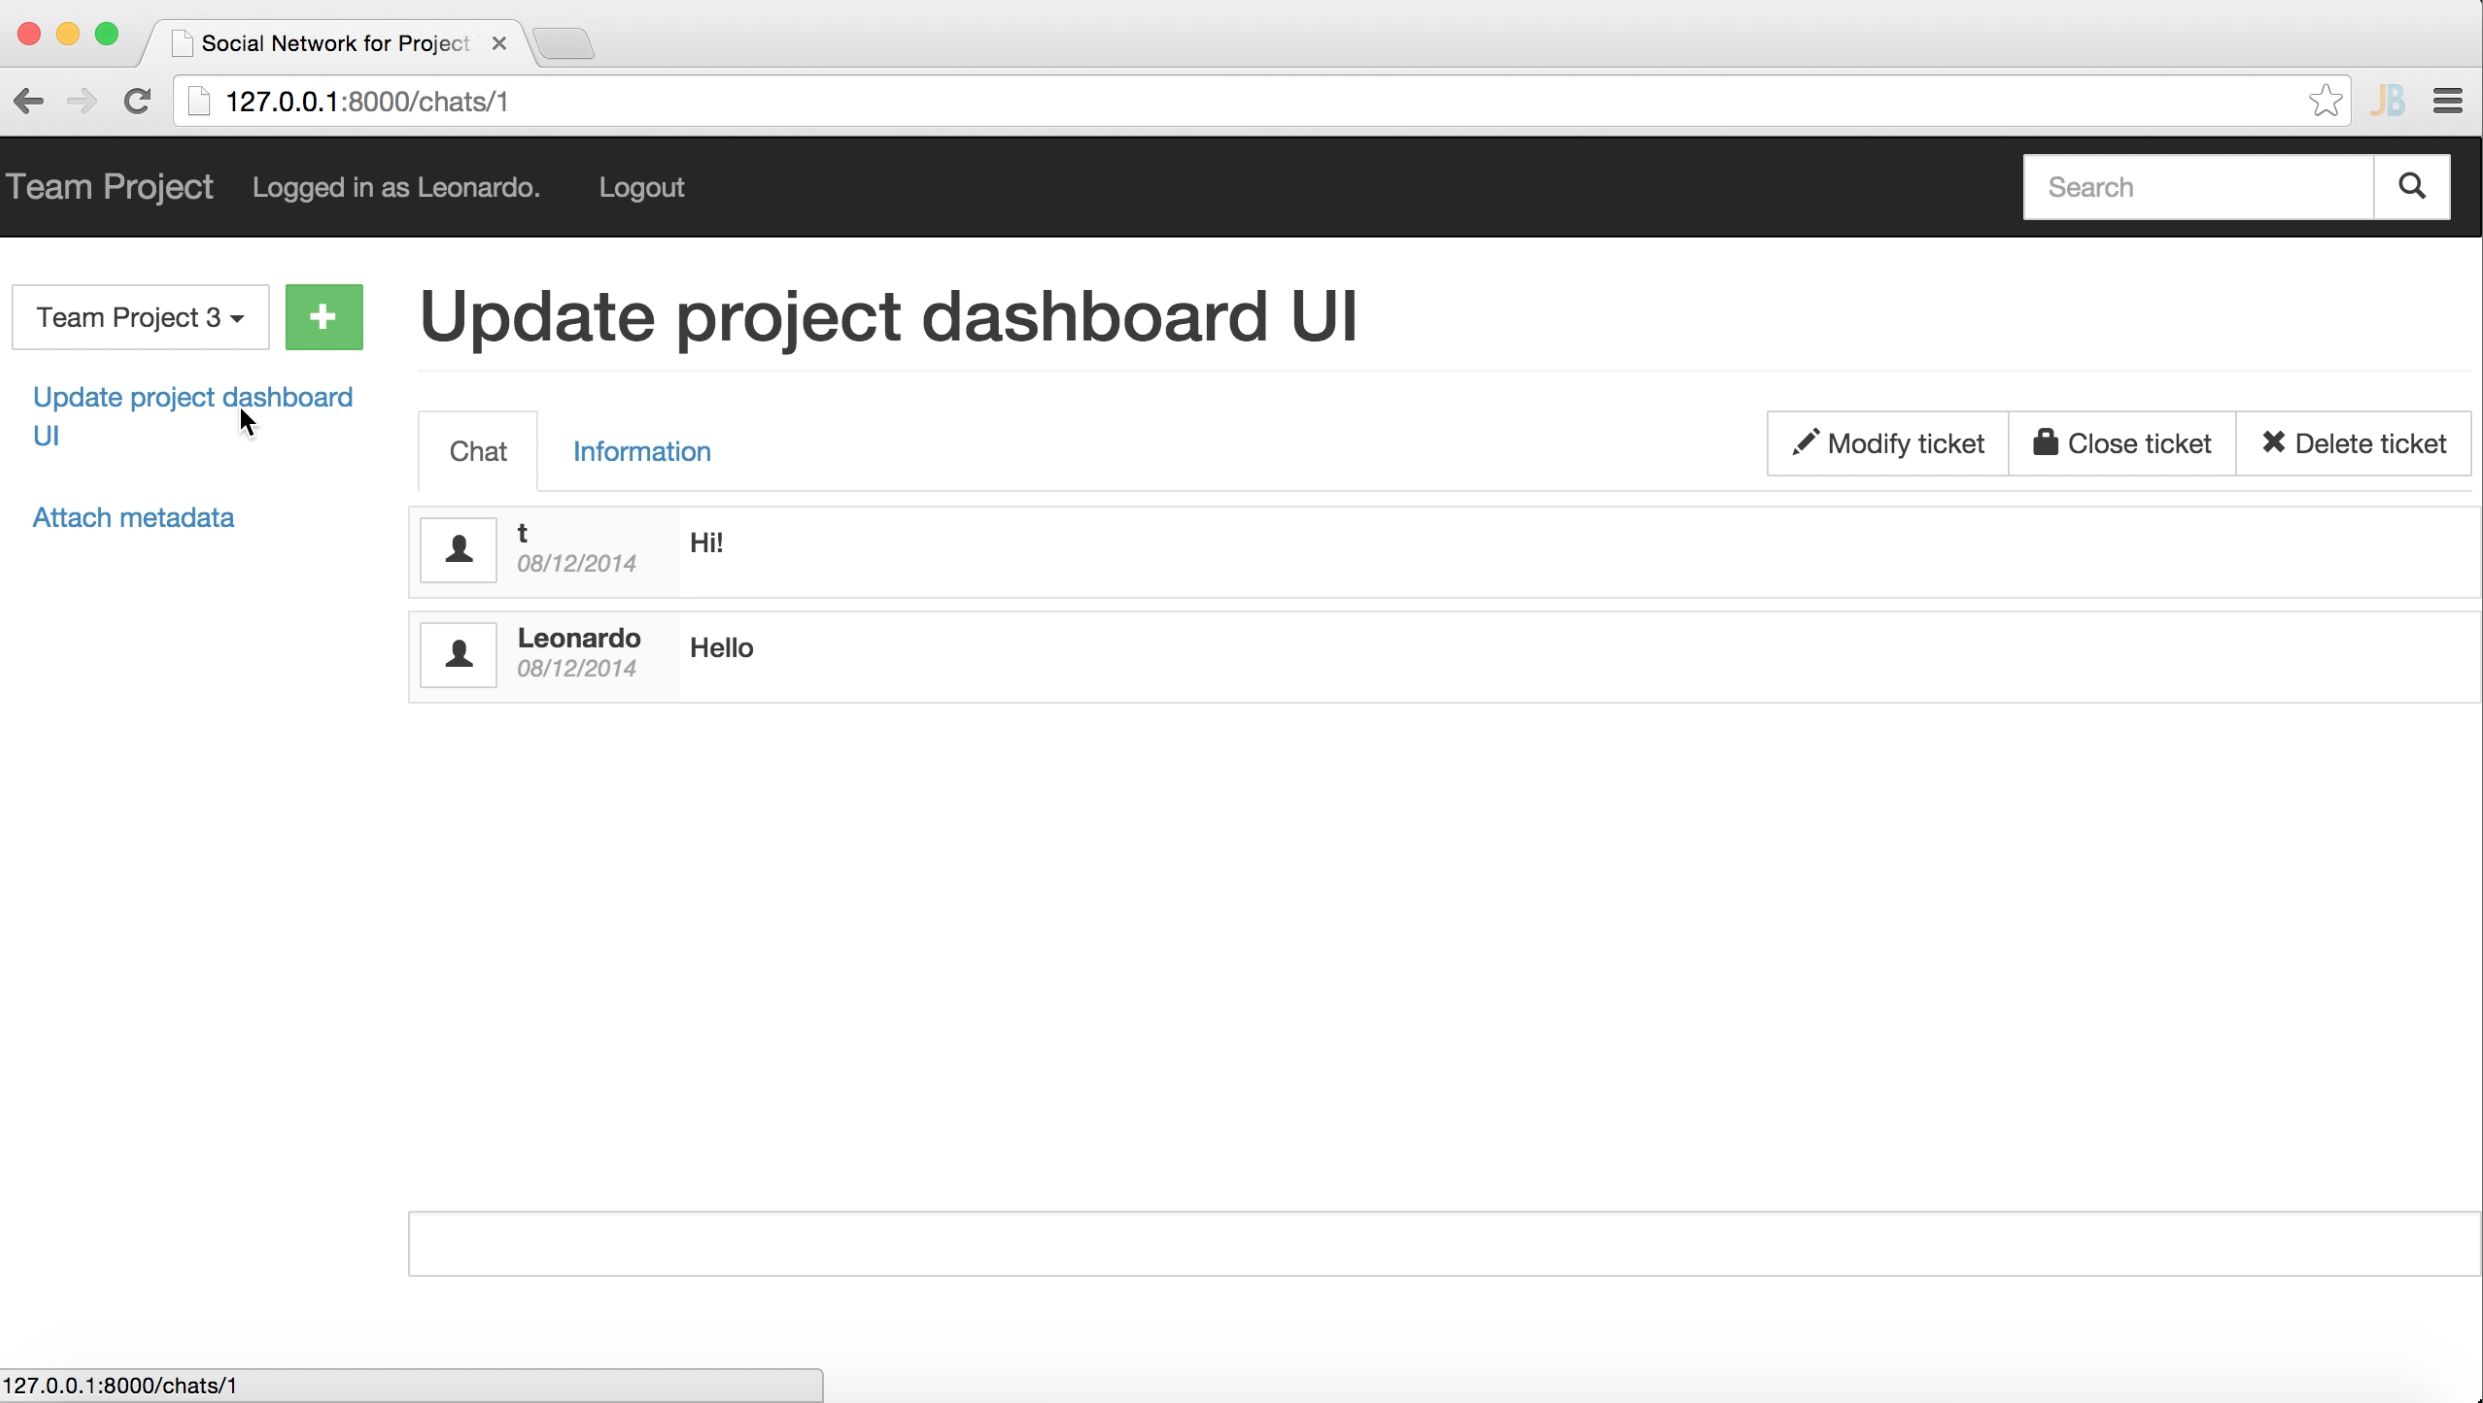
\includegraphics[scale=0.3]{prototype}
\caption{Prototype}
\label{figure:prototype}
\end{figure}

The aim of developing the prototype was to create a basic proof-of-concept to display, which could then be build upon instead of implementing multiple user stories, resulting in a fragmented program with many isolated features but no overall functionality.  The final demonstration therefore lacked the polish and features to be delivered by the end of the project. The tradeoff for this was that features were much easier to implement in the future, and solid groundwork had been made which the team could now build upon. 


%----------------------------------------------------------------------------
\section{Metadata}
\label{metadata}

The ability to attach metadata to conversations is a core feature, and one which differentiates the software from standard instant messaging applications. It is also the feature that makes the application suitable for use as a project management tool. Metadata provides essential information for developers and managers regarding a conversation, and is accessible through the information tab. Metadata is a crucial feature of the final product, so a prominent position was given in the UI. A dropdown menu to the right of the screen, shown in \autoref{figure:metadata1}, allowed for the easy addition of six metadata types through a menu shown in \autoref{figure:metadata2}.

\begin{figure}
\centering
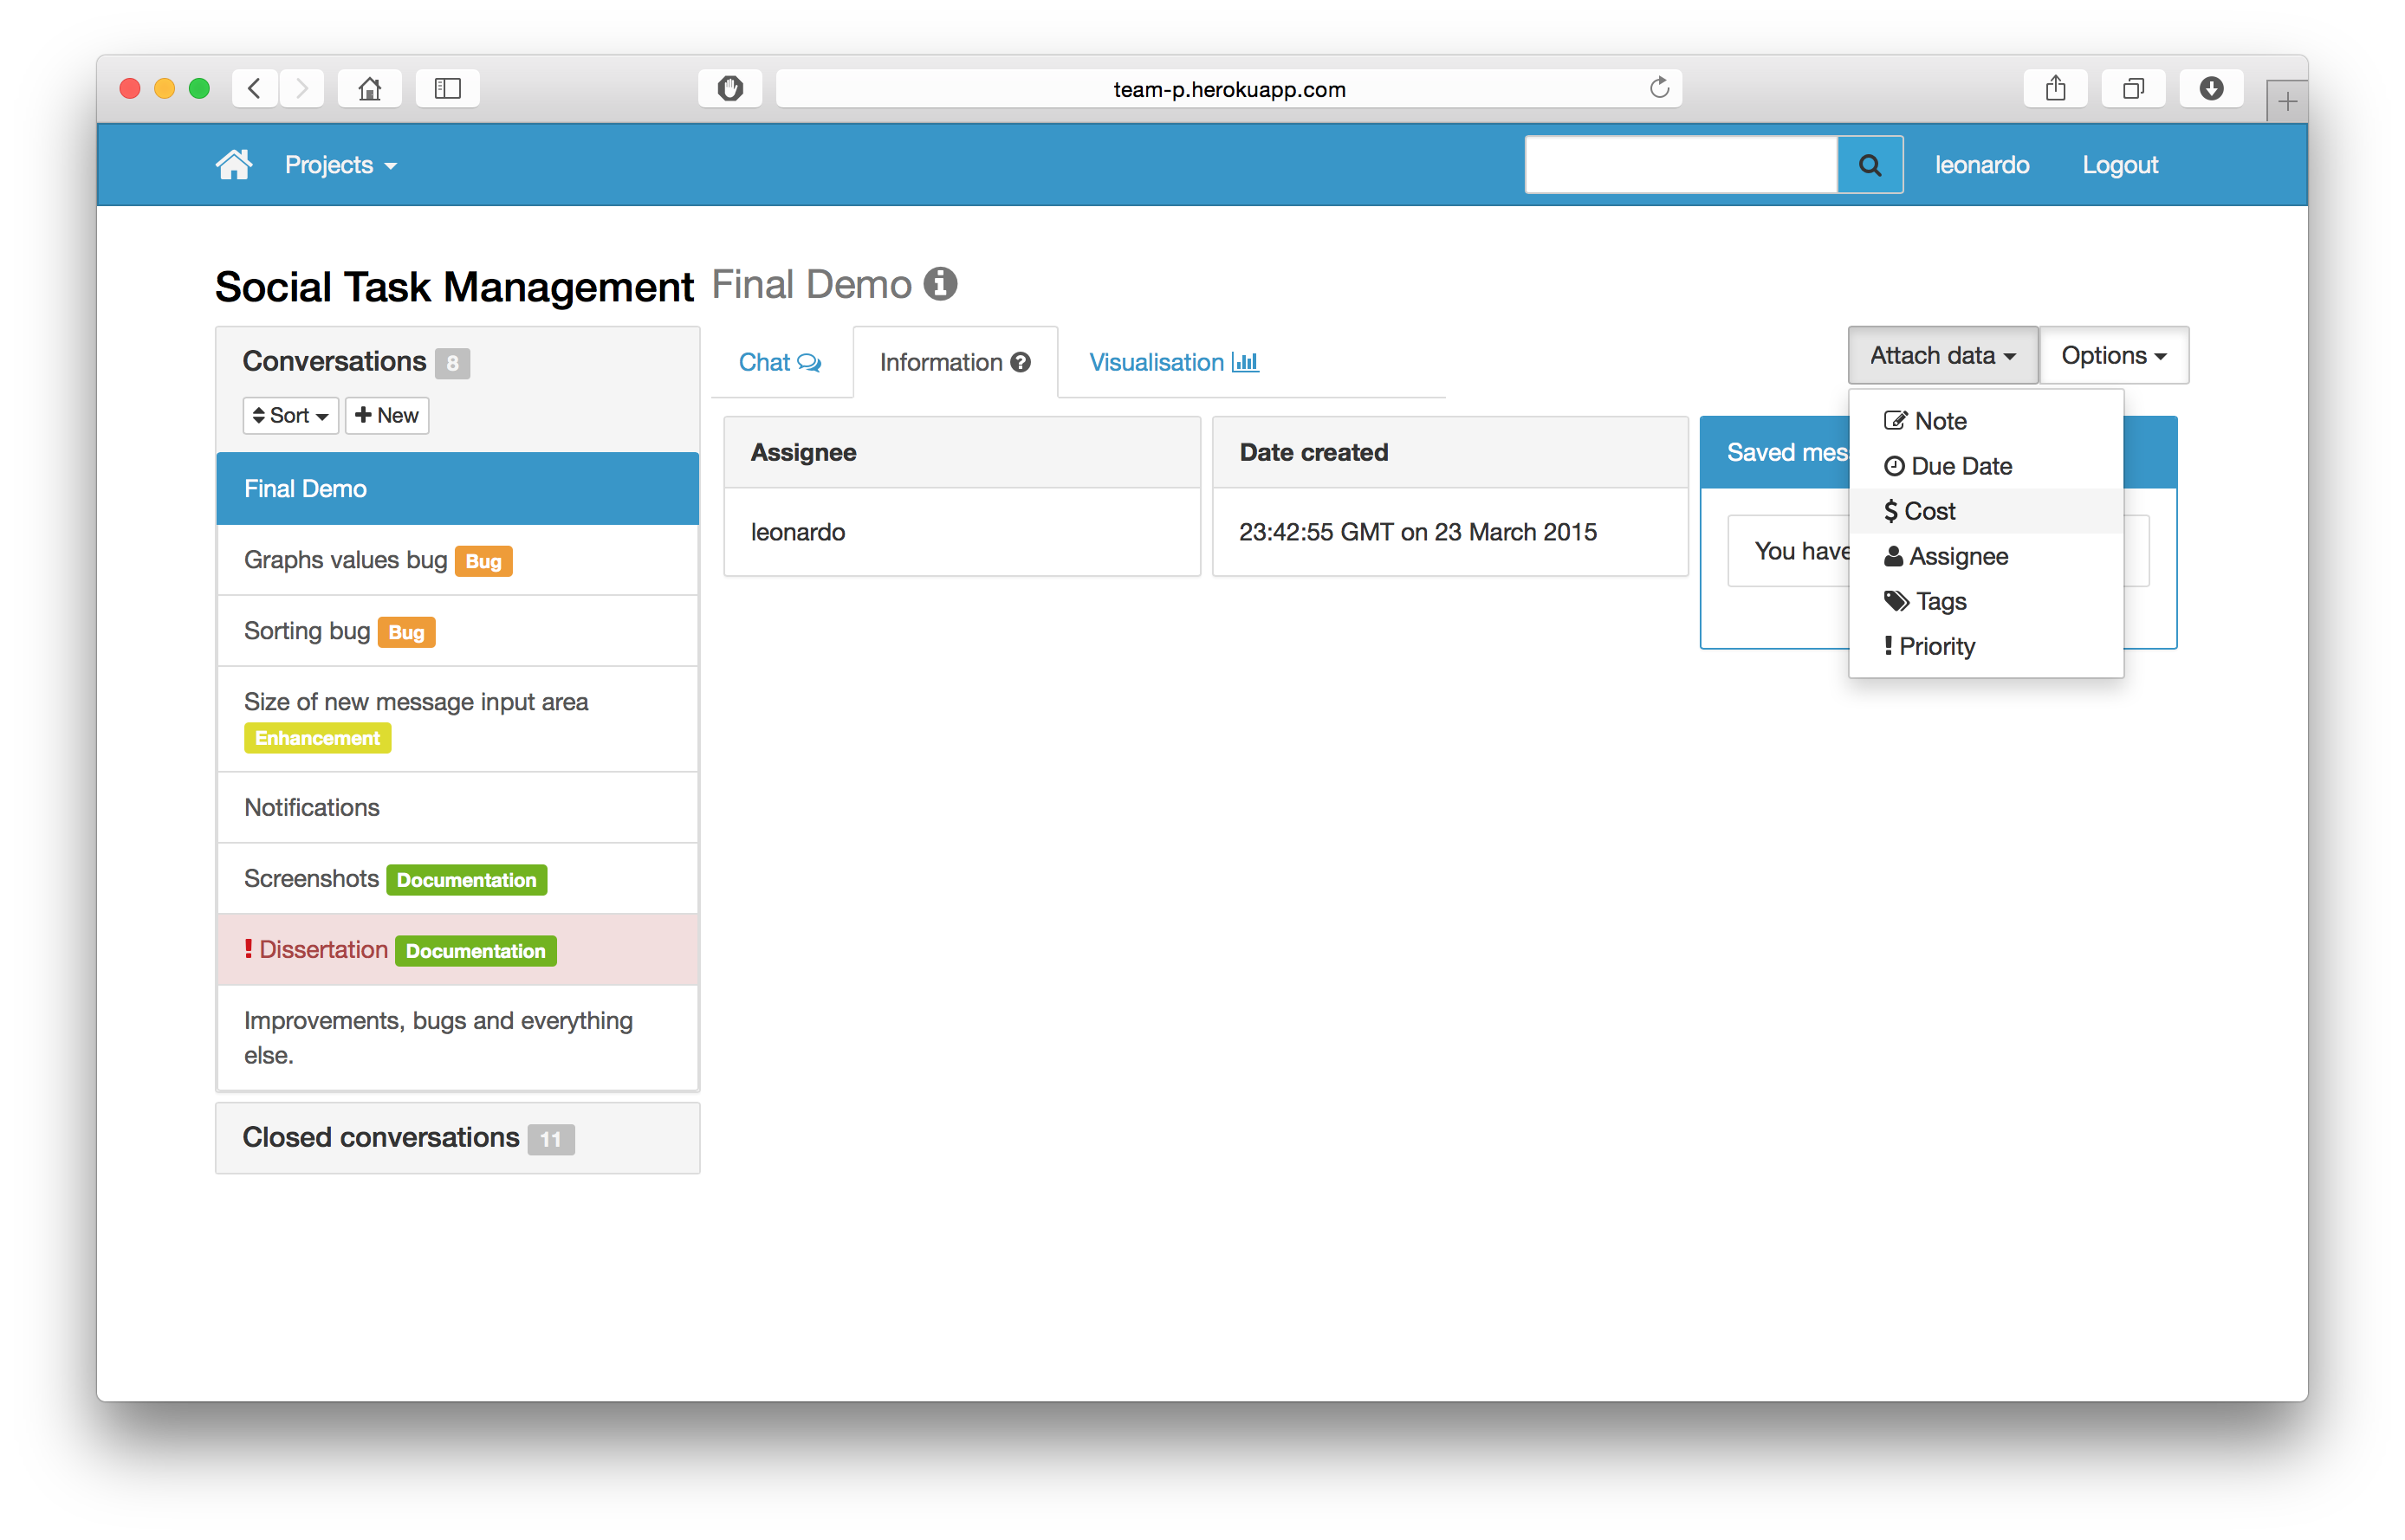
\includegraphics[scale=0.3]{dropdownMenu}
\caption{Add metadata dropdown menu}
\label{figure:metadata1}
\end{figure}

\begin{figure}
\centering
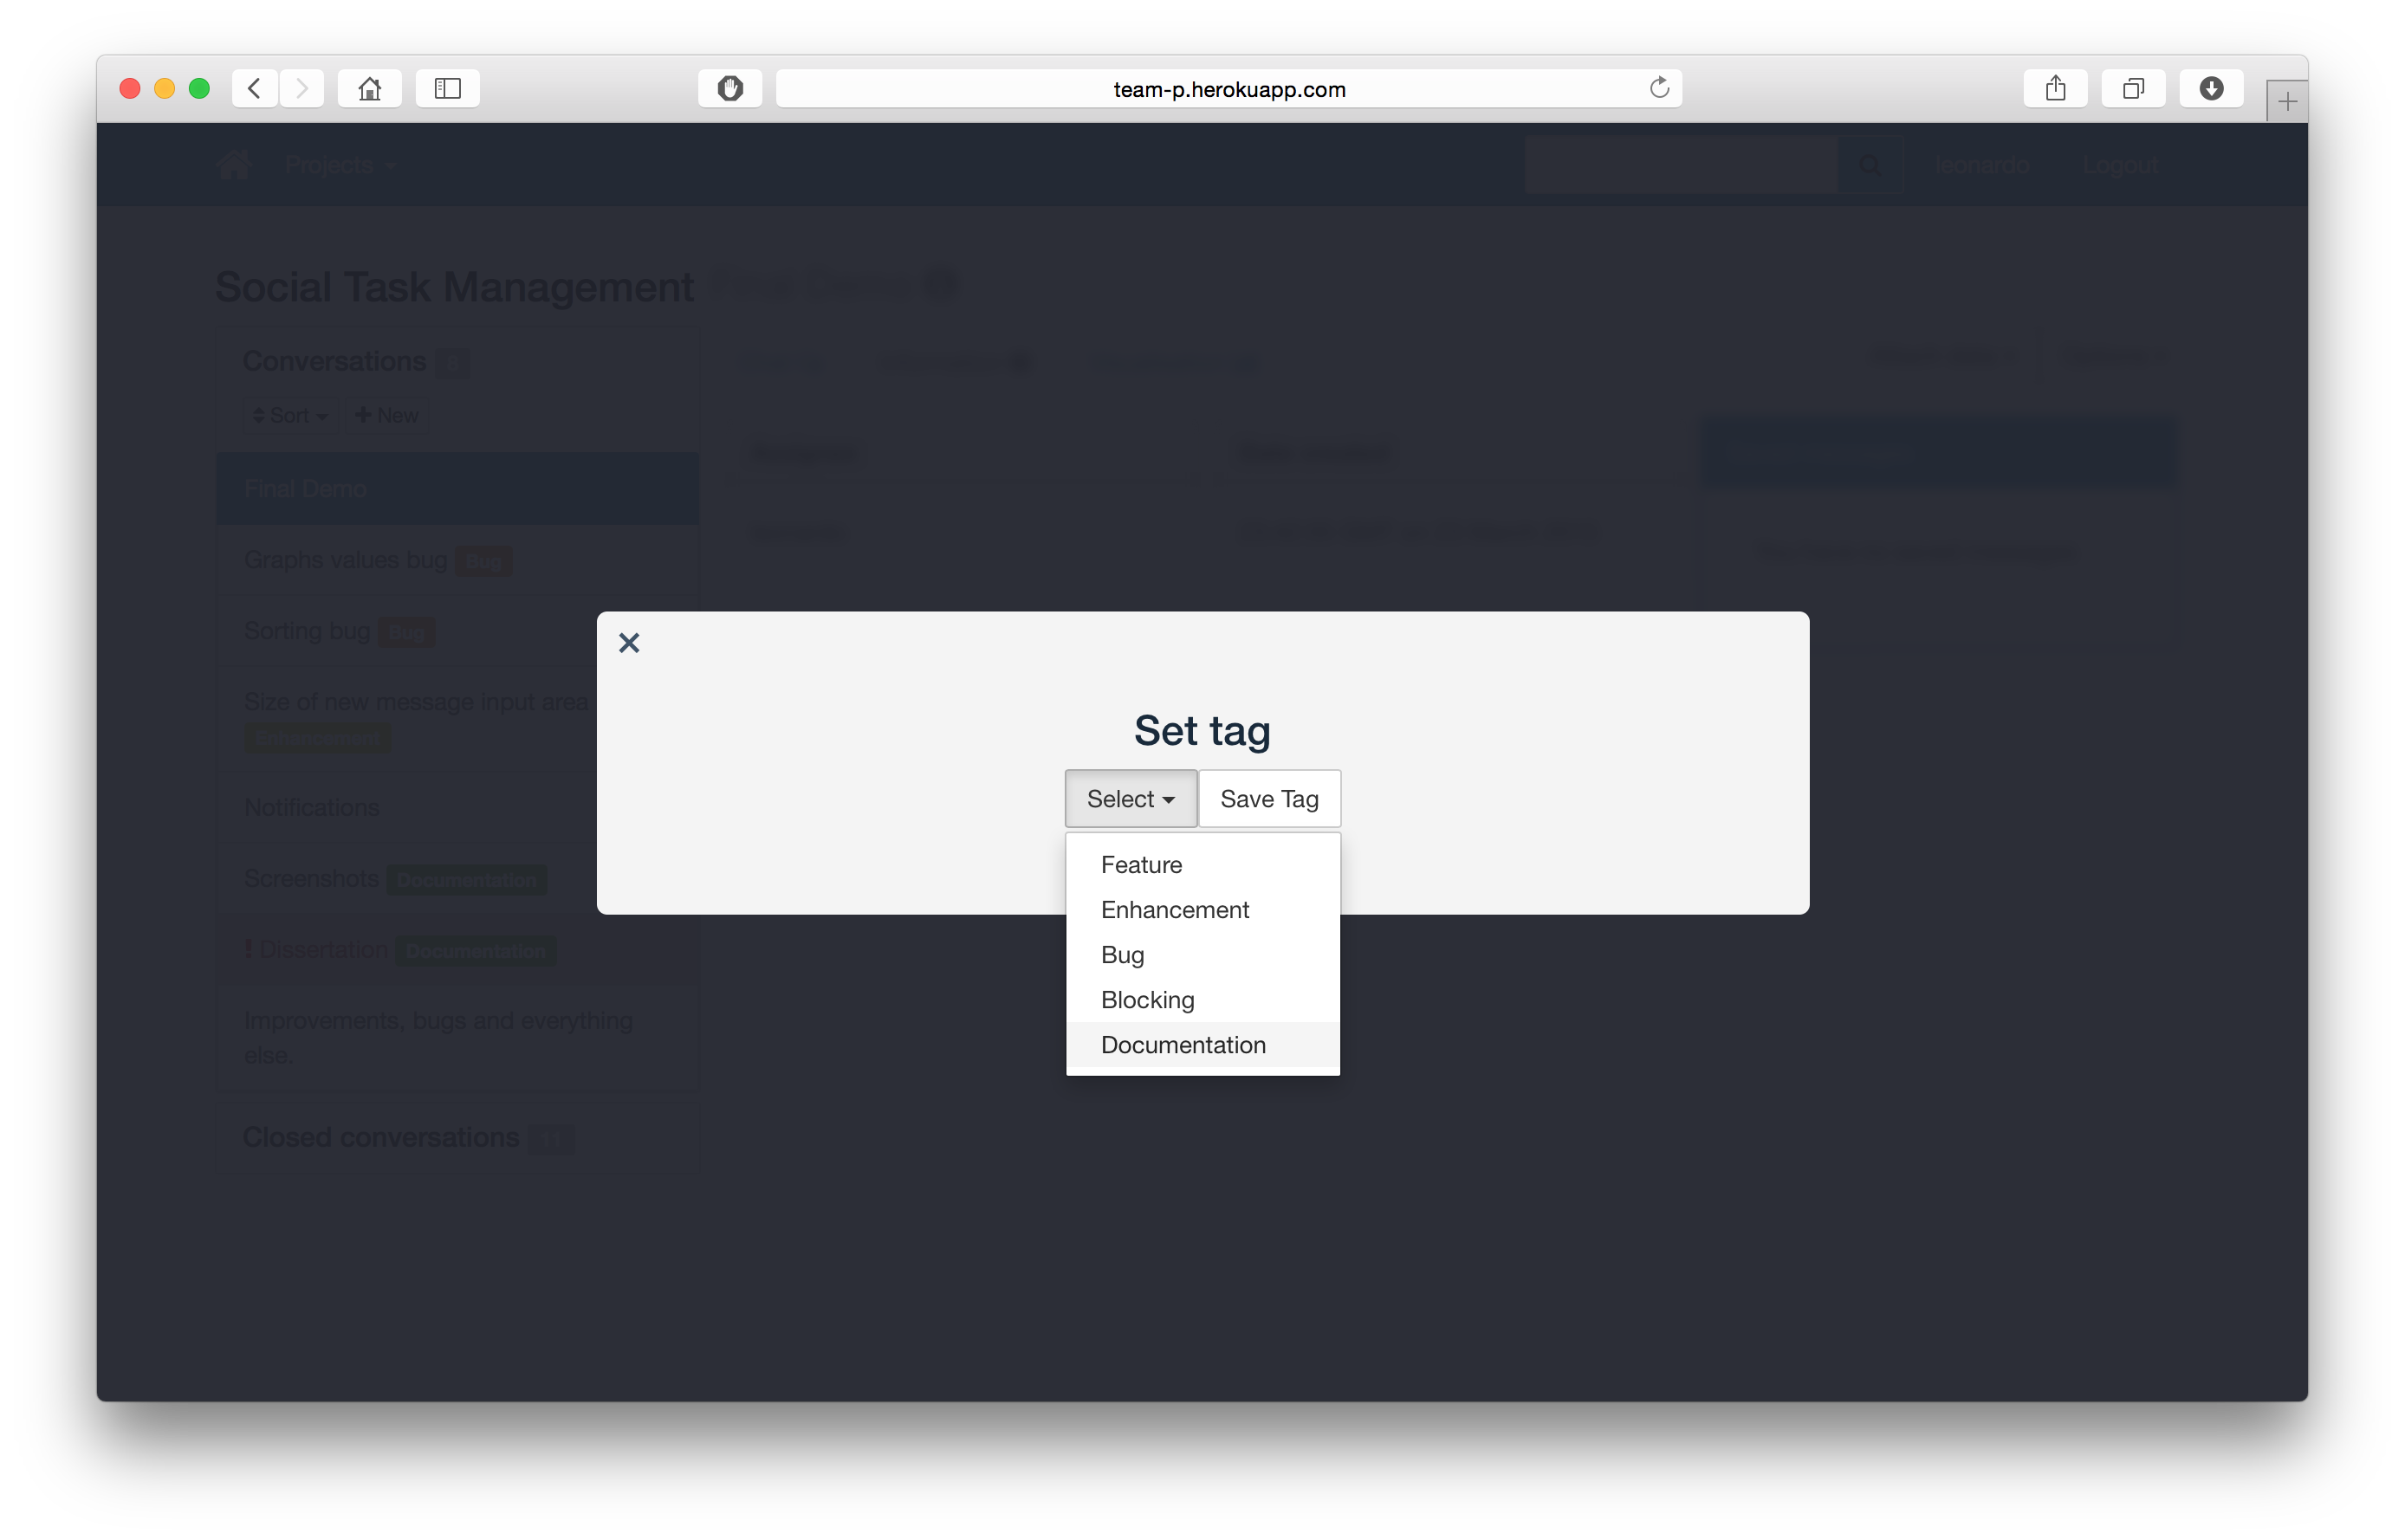
\includegraphics[scale=0.3]{addMetadata}
\caption{Add metadata}
\label{figure:metadata2}
\end{figure}

\begin{figure}
\centering
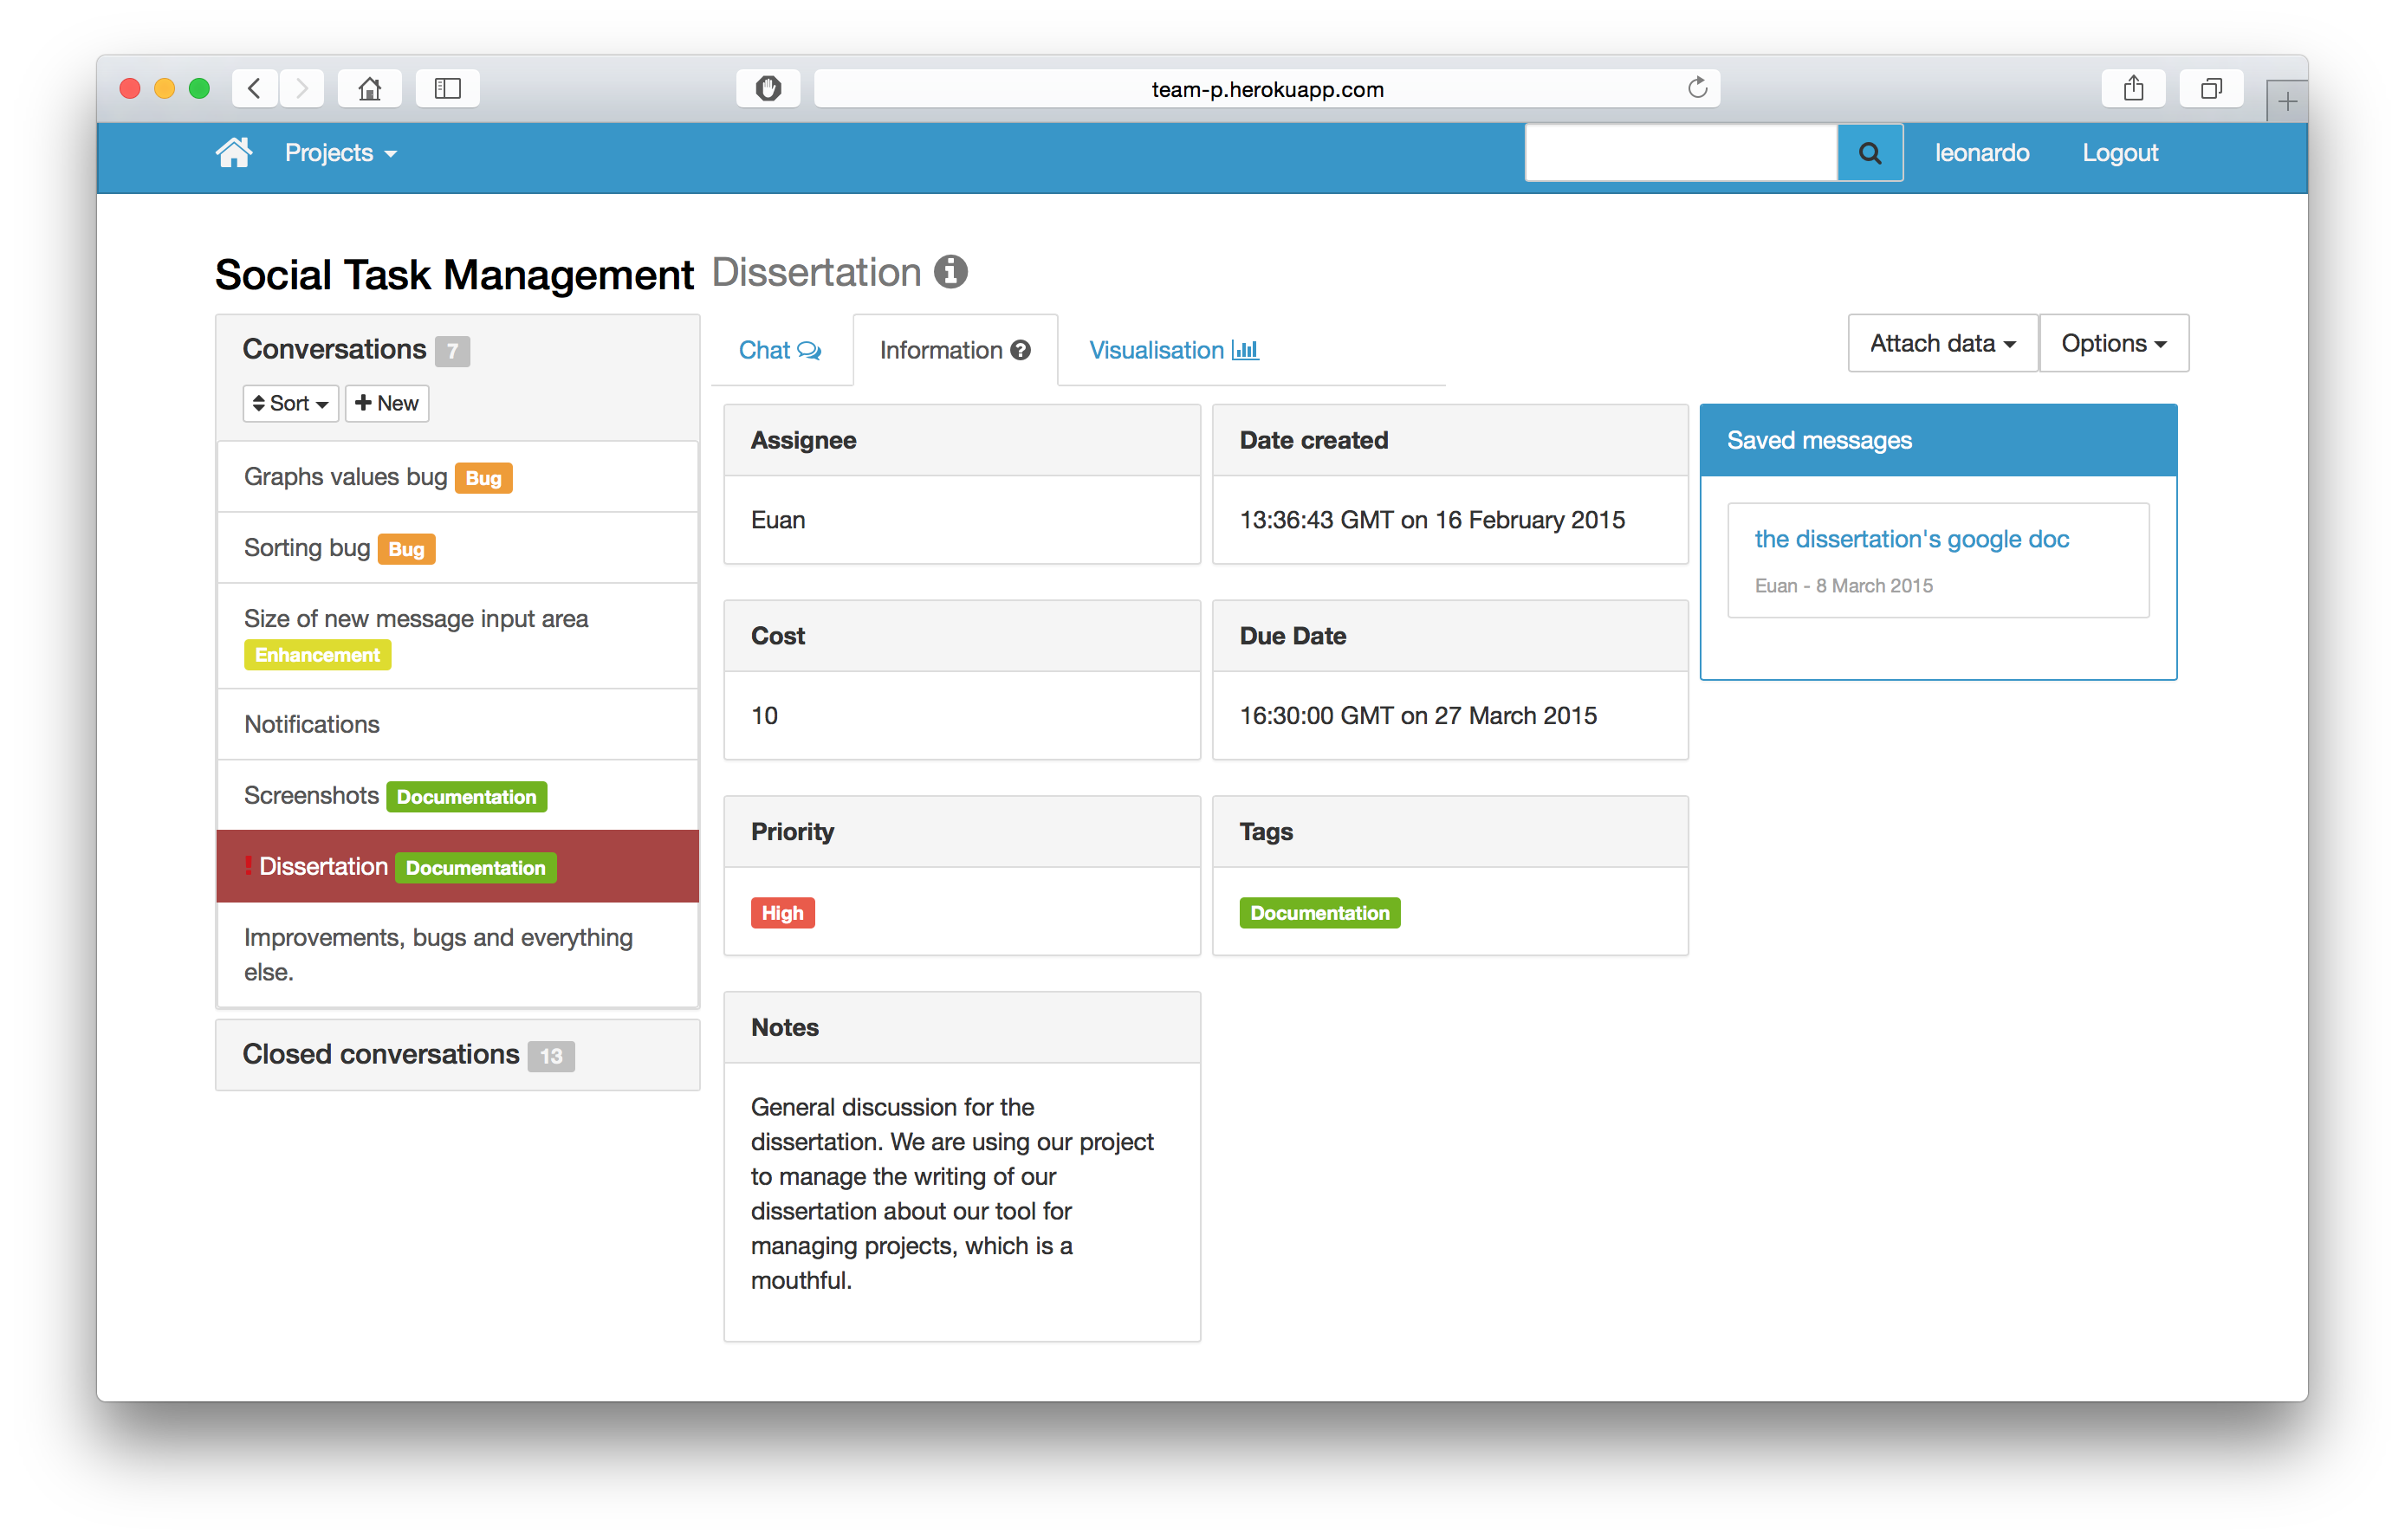
\includegraphics[scale=0.3]{allmetadata}
\caption{All metadata}
\label{figure:metadata3}
\end{figure}


The metadata types are defined below and shown in \autoref{figure:metadata3}.

\begin{itemize}
\item \textit{Assignee} \par
The user that creates the conversation is its assignee by default. Users can edit this later and choose from a dropdown list another user to be assigned.
\item \textit{Cost} \par
 A decimal field which can be used flexibly by development teams to indicate the effort required to complete a task. The field is unitless and therefore does not enforce a specific cost prediction method. Therefore, teams can define their own baseline from which to judge the cost of a specific task.
 \item \textit{Due Date} \par
The date and time before which the issue discussed in the conversation should be resolved.
\item \textit{Notes} \par
A text field which is primarily used for linking to resources relating to the conversation. This field supports Markdown notation, meaning that teams can use it to store almost any type of well formatted miscellaneous information.
\item \textit{Priority} \par
This can be used to indicate the importance of a conversation. This field can contain any one of the values: “Low”, “Medium”, or “High”. Conversations marked as high priority are displayed with a red background in the conversations list.
\item \textit{Tags} \par
Users can set tags for a conversation. Every tag has a special label colour and is displayed beside of conversation title to make it easy to identify the nature of the conversation.
\end{itemize}
 


%----------------------------------------------------------------------------
\section{Statistics}
\label{statistics}

The visualisation of statistics regarding a team’s activity was deemed an important feature of the product. Providing metrics to users allows for the identification of successes and failures within a project. Although the statistics provided cannot provide an absolute indication of the exact state of the project, they may provide hints to project managers of issues regarding progress or levels of developer contribution. A conversation which has been open for a week without any activity may indicate that an issue is being ignored, for example, and the graphs intend to aid in identifying situations like this.

Three graphs were implemented to show a proof-of-concept of how visually representing information would enhance a user’s understanding of their project. 
All visualisations were implemented as simple bar charts. It was found that, in all three cases, the data being displayed was a mapping of ordinal data and quantitative value. Users’ familiarity with bar charts made them an obvious choice for representing the site’s data. 
The graphs provided were:

\begin{itemize}
\item Messages sent per user in a conversation
\item Messages sent per user in a project
\item Messages contained in each conversation in a project
\end{itemize}

These graphs were intended to show user participation and chat activity in a way that would allow an observer to judge the importance of different chats within the system, and to see the contributions a user was making on both a project level and within specific conversations.

The graphs, shown in \autoref{figure:graphs1} and \autoref{figure:graphs2}, were constructed using the D3 \cite{site:d3} Javascript library. D3 allowed for the creation of graphs with relative ease, powered by the conversation data from Firebase.
In addition, D3 allowed for the creation of tooltips which contained data regarding points on the graphs. It was identified that containing exact data on each bar of the graphs could make them cluttered, making data more difficult to understand at a glance. Therefore, the graph was designed to provide a simple visualisation of data, and tooltips would explain the data provided more when points on the graph were hovered over. 

\begin{figure}
\centering
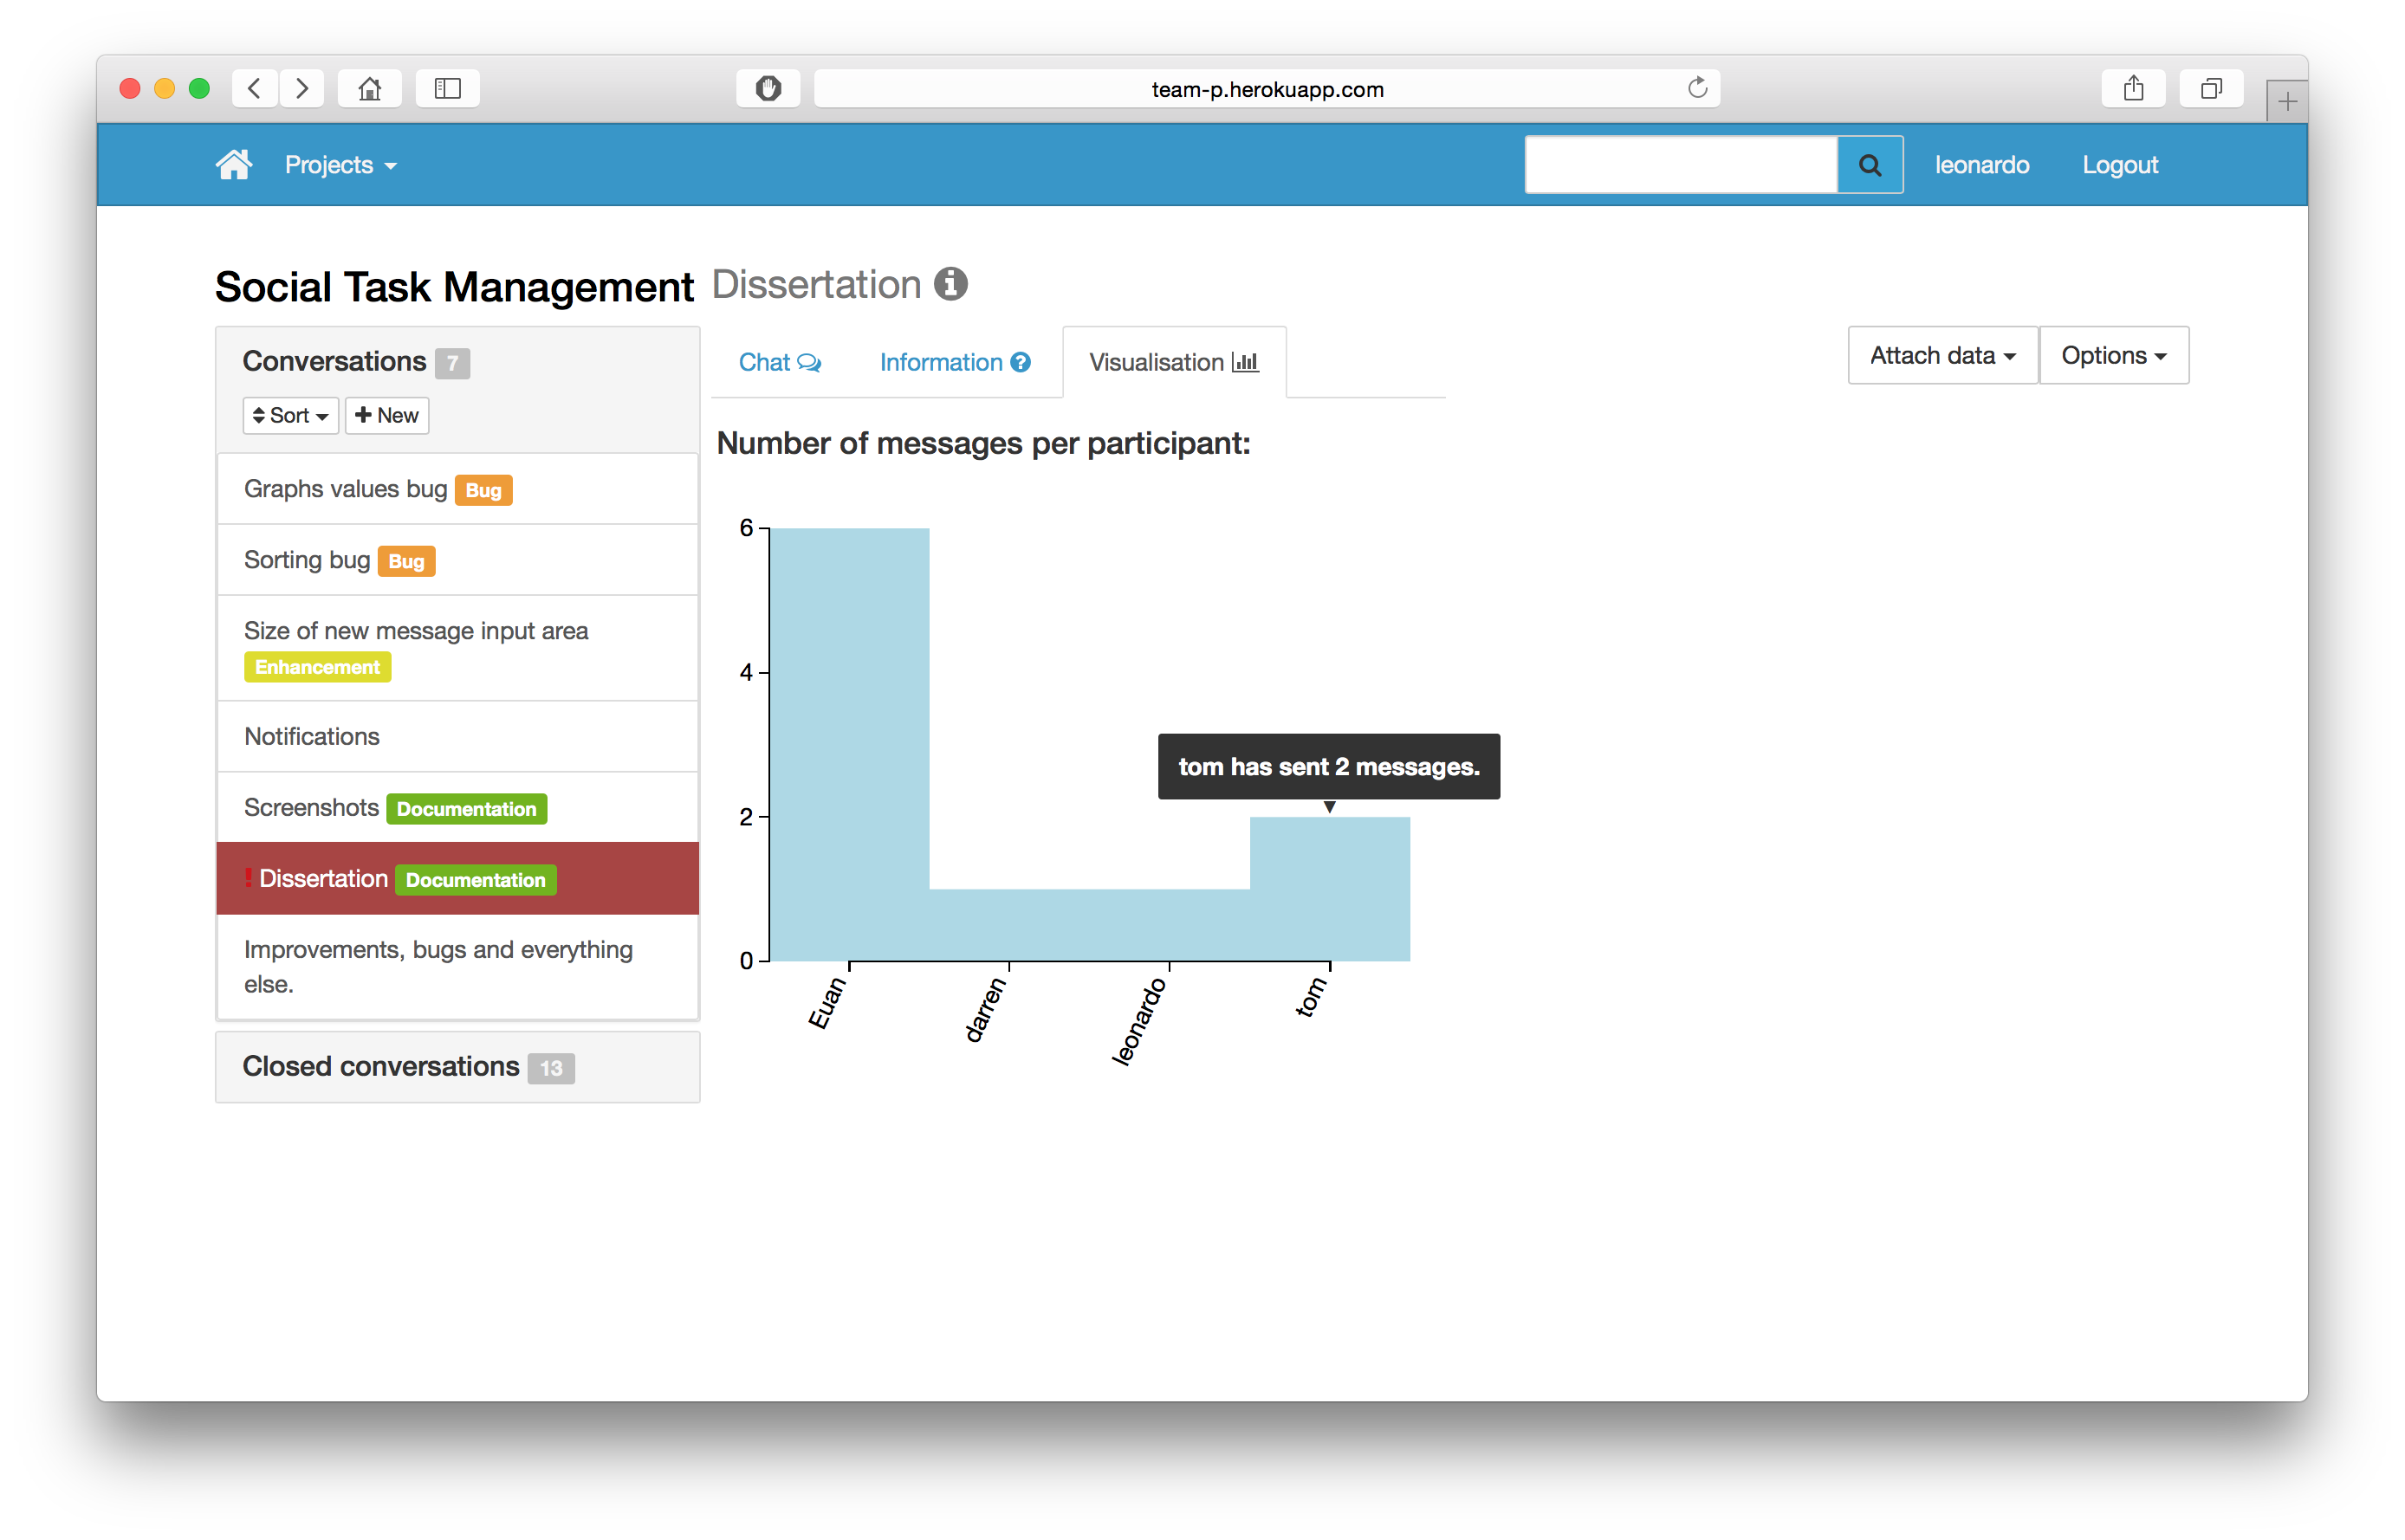
\includegraphics[scale=0.3]{graphs1}
\caption{Chat graph}
\label{figure:graphs1}
\end{figure}

\begin{figure}
\centering
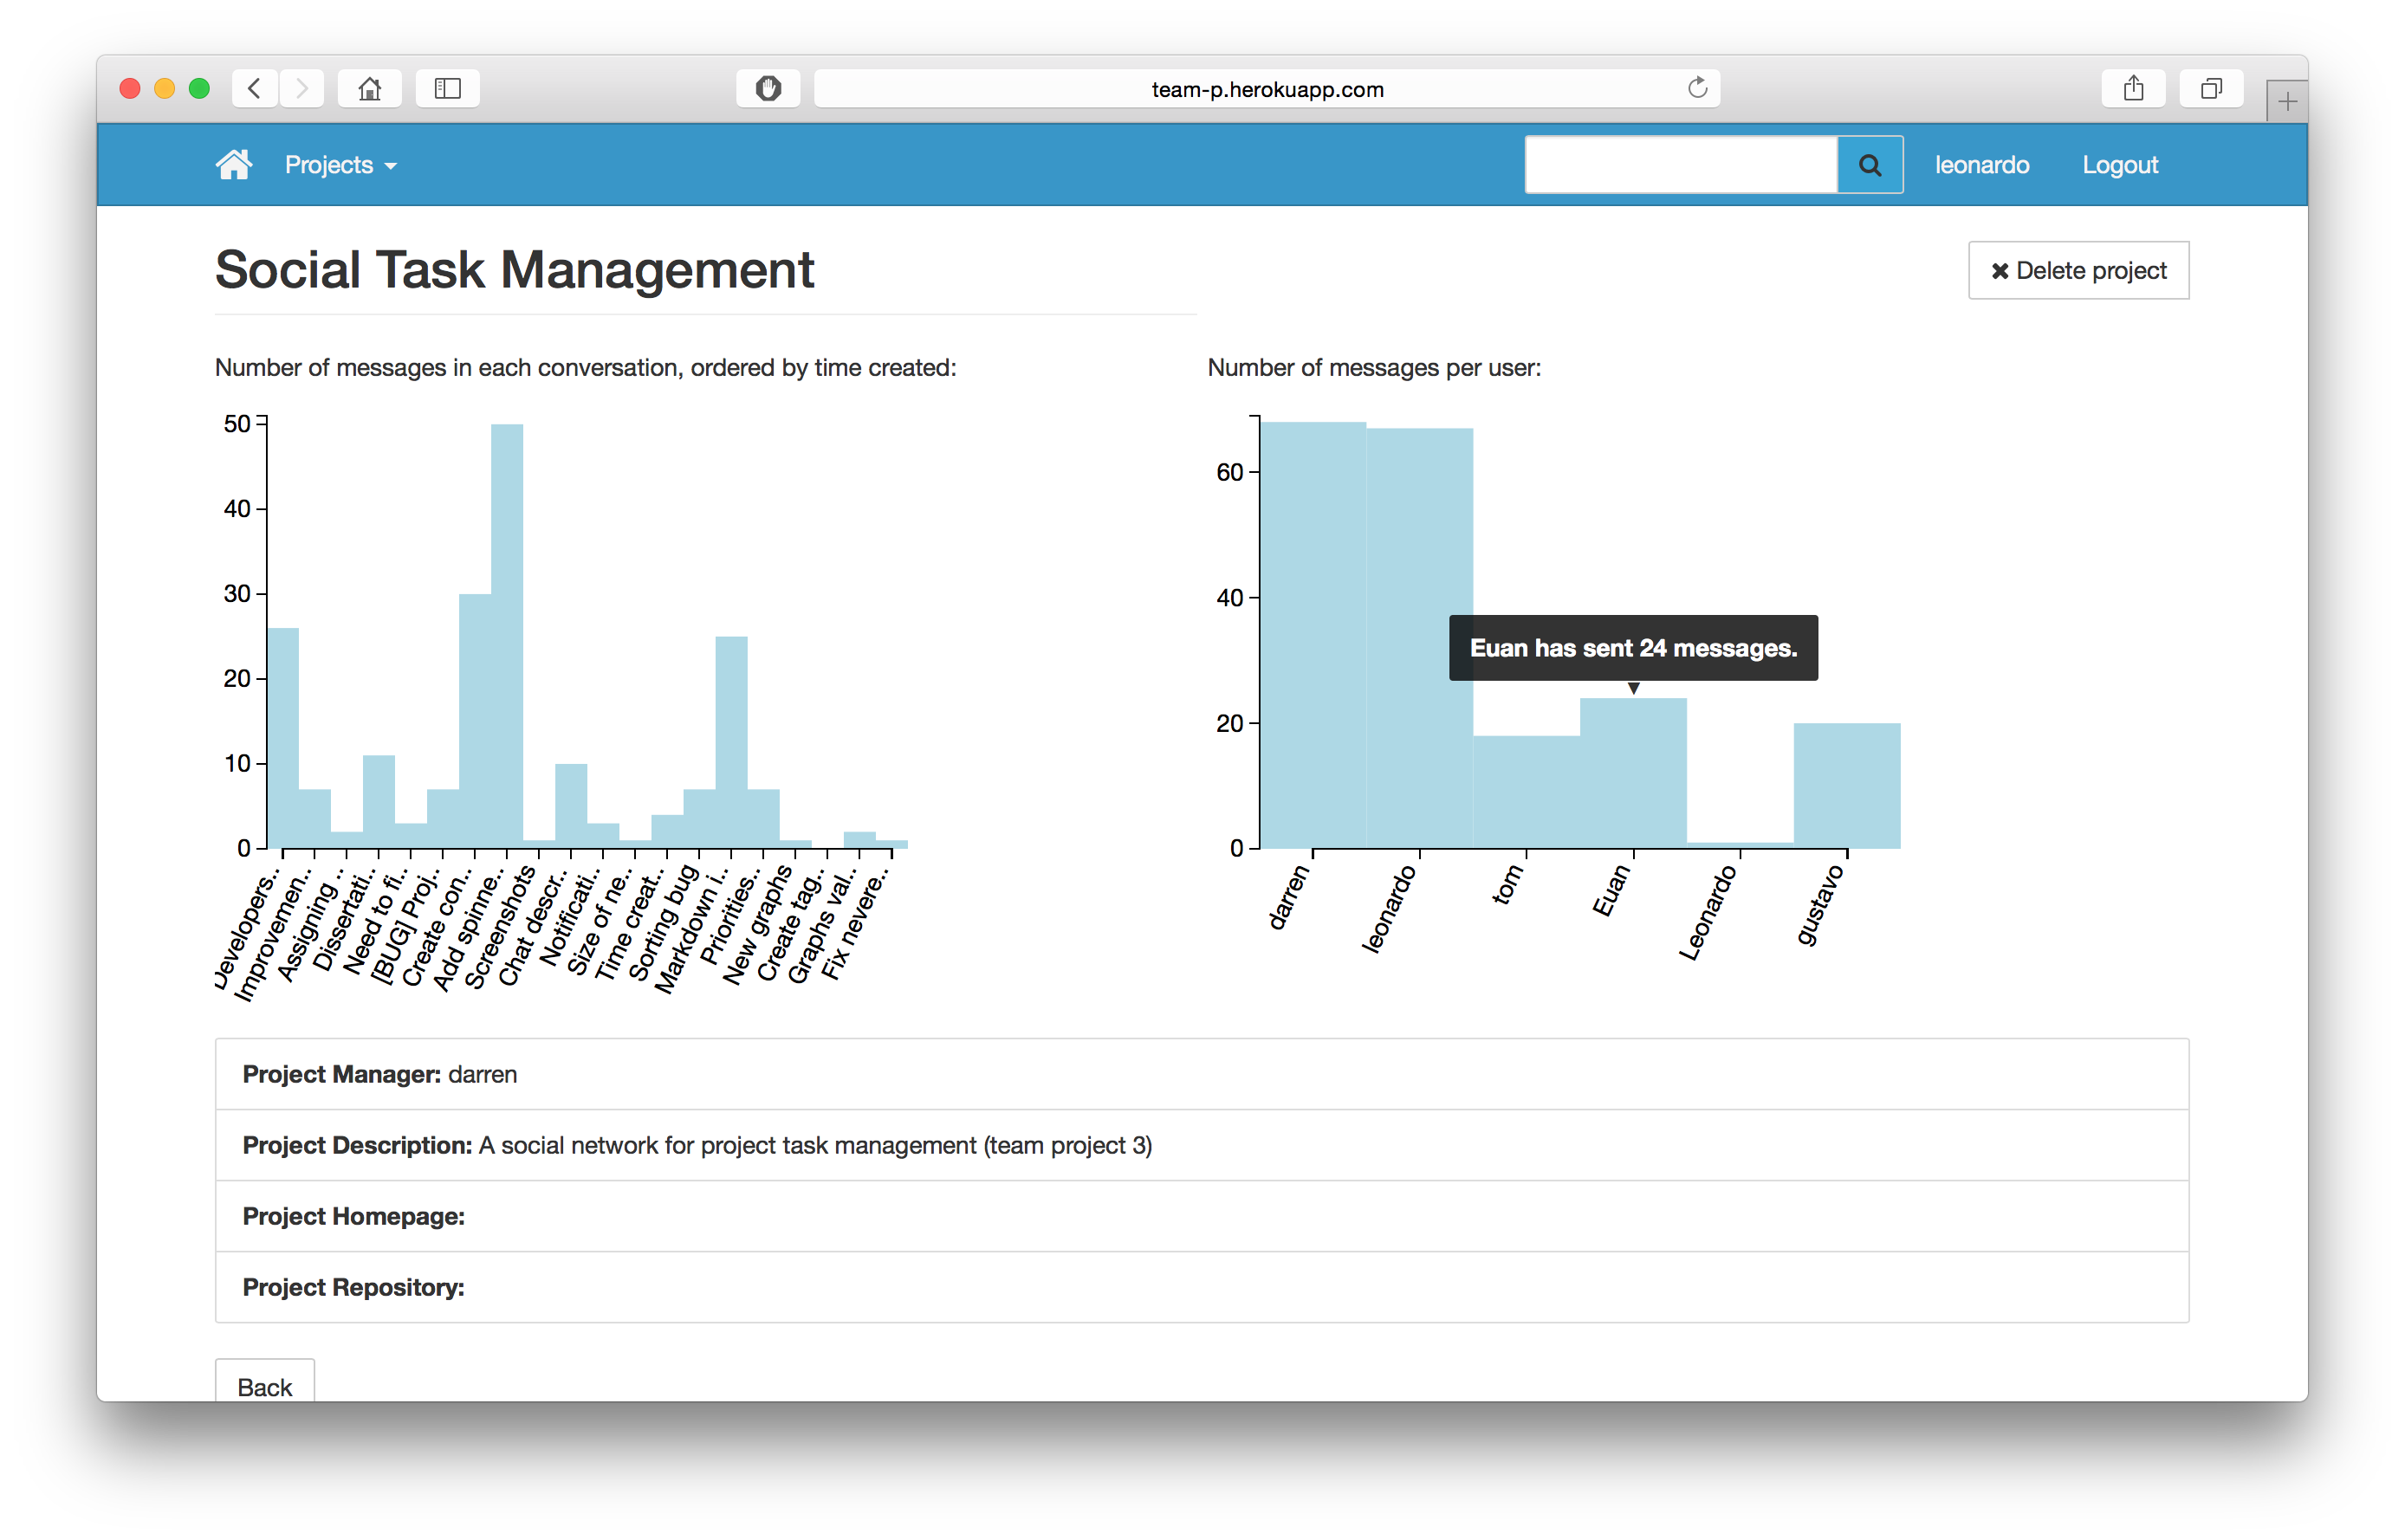
\includegraphics[scale=0.3]{graphs2}
\caption{Project graphs}
\label{figure:graphs2}
\end{figure}


%----------------------------------------------------------------------------
\section{Additional Features}
\label{dog}
With the software being aimed at software development projects, the team was in an excellent position to evaluate it themselves, by using it to manage the development. The following features were identified and then implemented after this self evaluation.

%----------------------------------------------------------------------------
\subsection{Notifications}
\label{notifications}

Users can participate in a significant number of different chats at the same time. Without a notification system, the user does not know when a chat had updates or if the user was mentioned in a conversation. The user could check each conversation manually, but it is non-practical and time consuming. In order to address this problem, the web notification feature was implemented.

The Notification API specification \cite{site:mdnNotifications} is currently under development, however the technology is supported by most of the modern browsers. Notifications consist of four main attributes: title, body, icon and tag (i.e. an identifier for the notification).

\begin{table}[h]
\begin{tabular}{|c|c|c|c|c|c|}
\hline
\textbf{Feature} & \textbf{Chrome} & \textbf{Firefox (Gecko)} & \textbf{Internet Explorer} & \textbf{Opera} & \textbf{Safari} \\ \hline
Basic Support    & 5 webkit 22     & 4.0 moz 22               & Not supported              & 25             & 6               \\ \hline
\end{tabular}
\end{table}

There is an script in the project that listens for updates in chats and when a change occurs, a new notification is created showing the id of the updated chat and the content of the new message and it is displayed to the user. While the notification is being displayed the user has three options: dismiss the notification, wait for the automatic closing time of ten seconds or click the notification and be redirected to the updated chat.

A listener awaits changes in any conversation. When the listener detects that a new message has been sent, a new notification is created showing the ID of the chat and the content of the new message. This notification is then sent to all participants, as shown in \autoref{figure:notification}. With the notification on screen, the user has three options: dismiss the notification, wait for the automatic closing time of ten seconds, or click the notification and be redirected to the conversation.

Currently, the notification system does not save updates from periods that the user was offline, however it addresses the issue whereby users would have to manually check for updates by delivering useful and real-time information to the user.


\begin{figure}[ht]
\centering
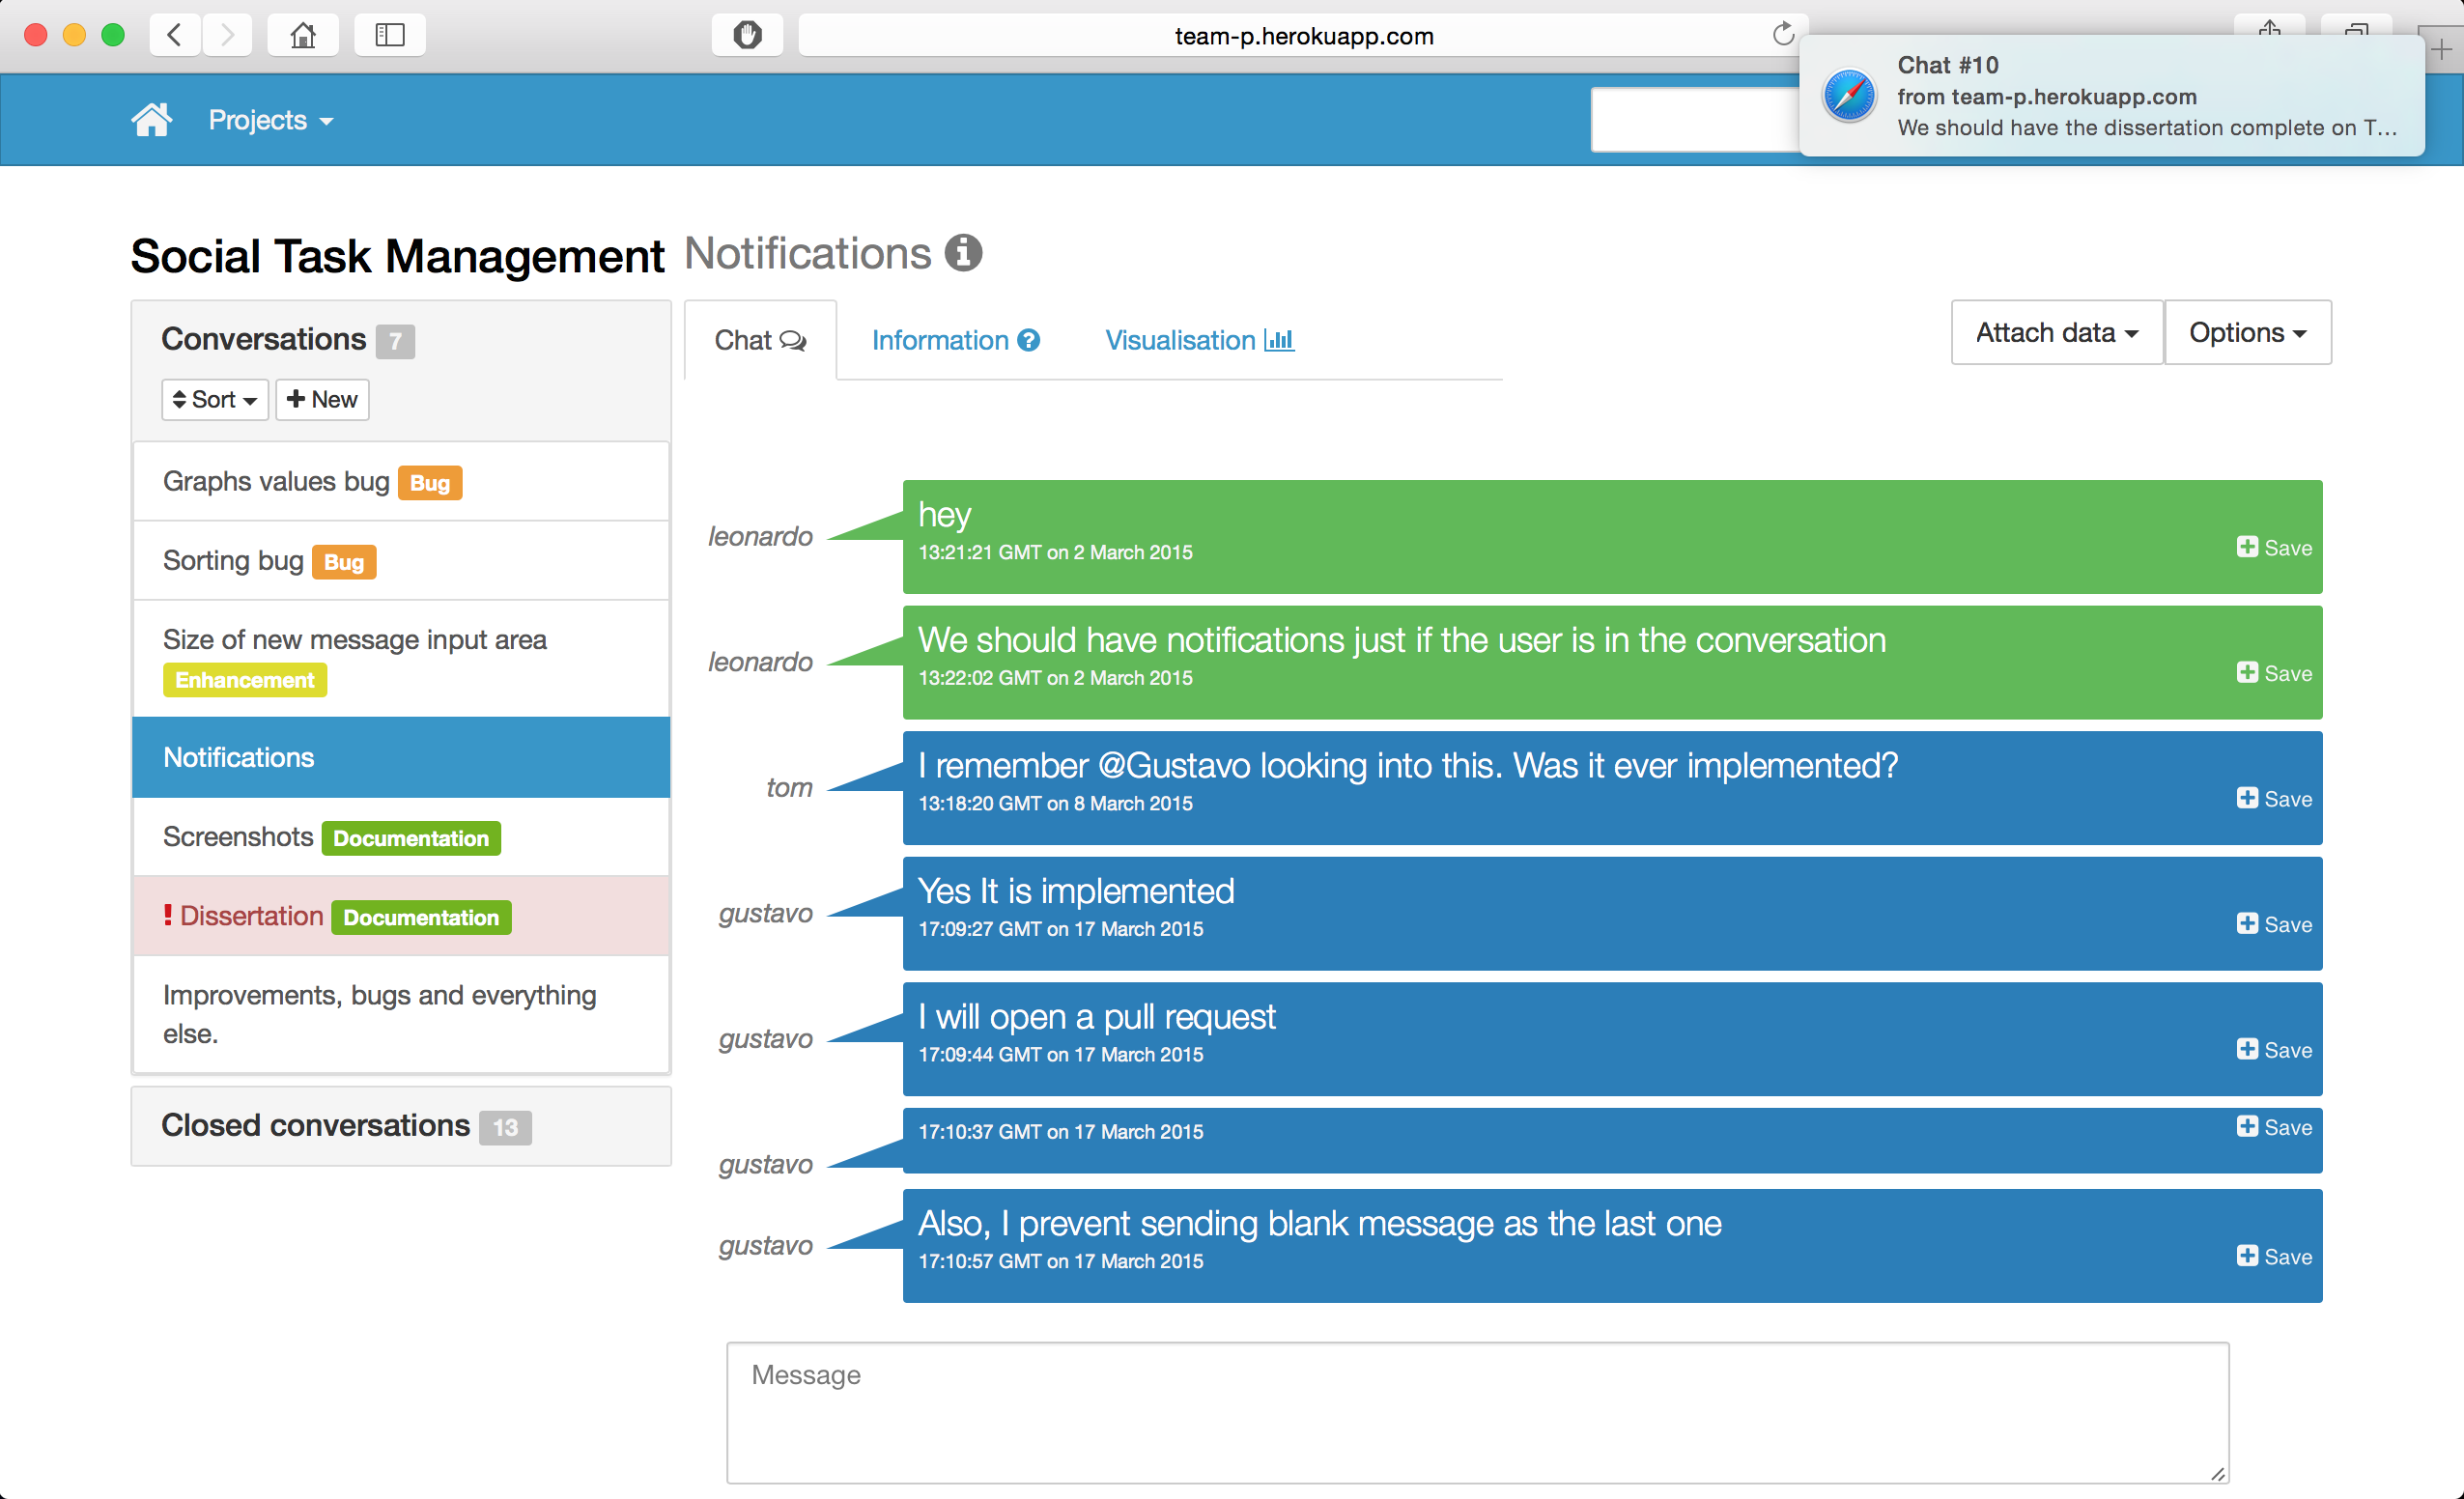
\includegraphics[scale=0.25]{notification}
\caption{Notification example}
\label{figure:notification}
\end{figure}


%----------------------------------------------------------------------------
\subsection{Saved Messages}
\label{savedMessages}

The number of messages in each chat can be considerable, so it can be quite difficult to locate messages of importance. The user could just add a note to avoid this problem, however this would involve copying the information from the message into the conversation notes. To do this each time important information was sent would be a slow and repetitive process. To solve this problem, the ability to save messages that are of value as metadata was added.

This feature provides a small button \autoref{fig:saveMessage} located in the bottom right corner of each message. If pressed, the message will be saved as an item of metadata in the information tab as shown on \autoref{fig:messageSaved}.

\begin{figure}[ht]
    \centering
    \begin{subfigure}[b]{0.48\textwidth}
	    \centering
		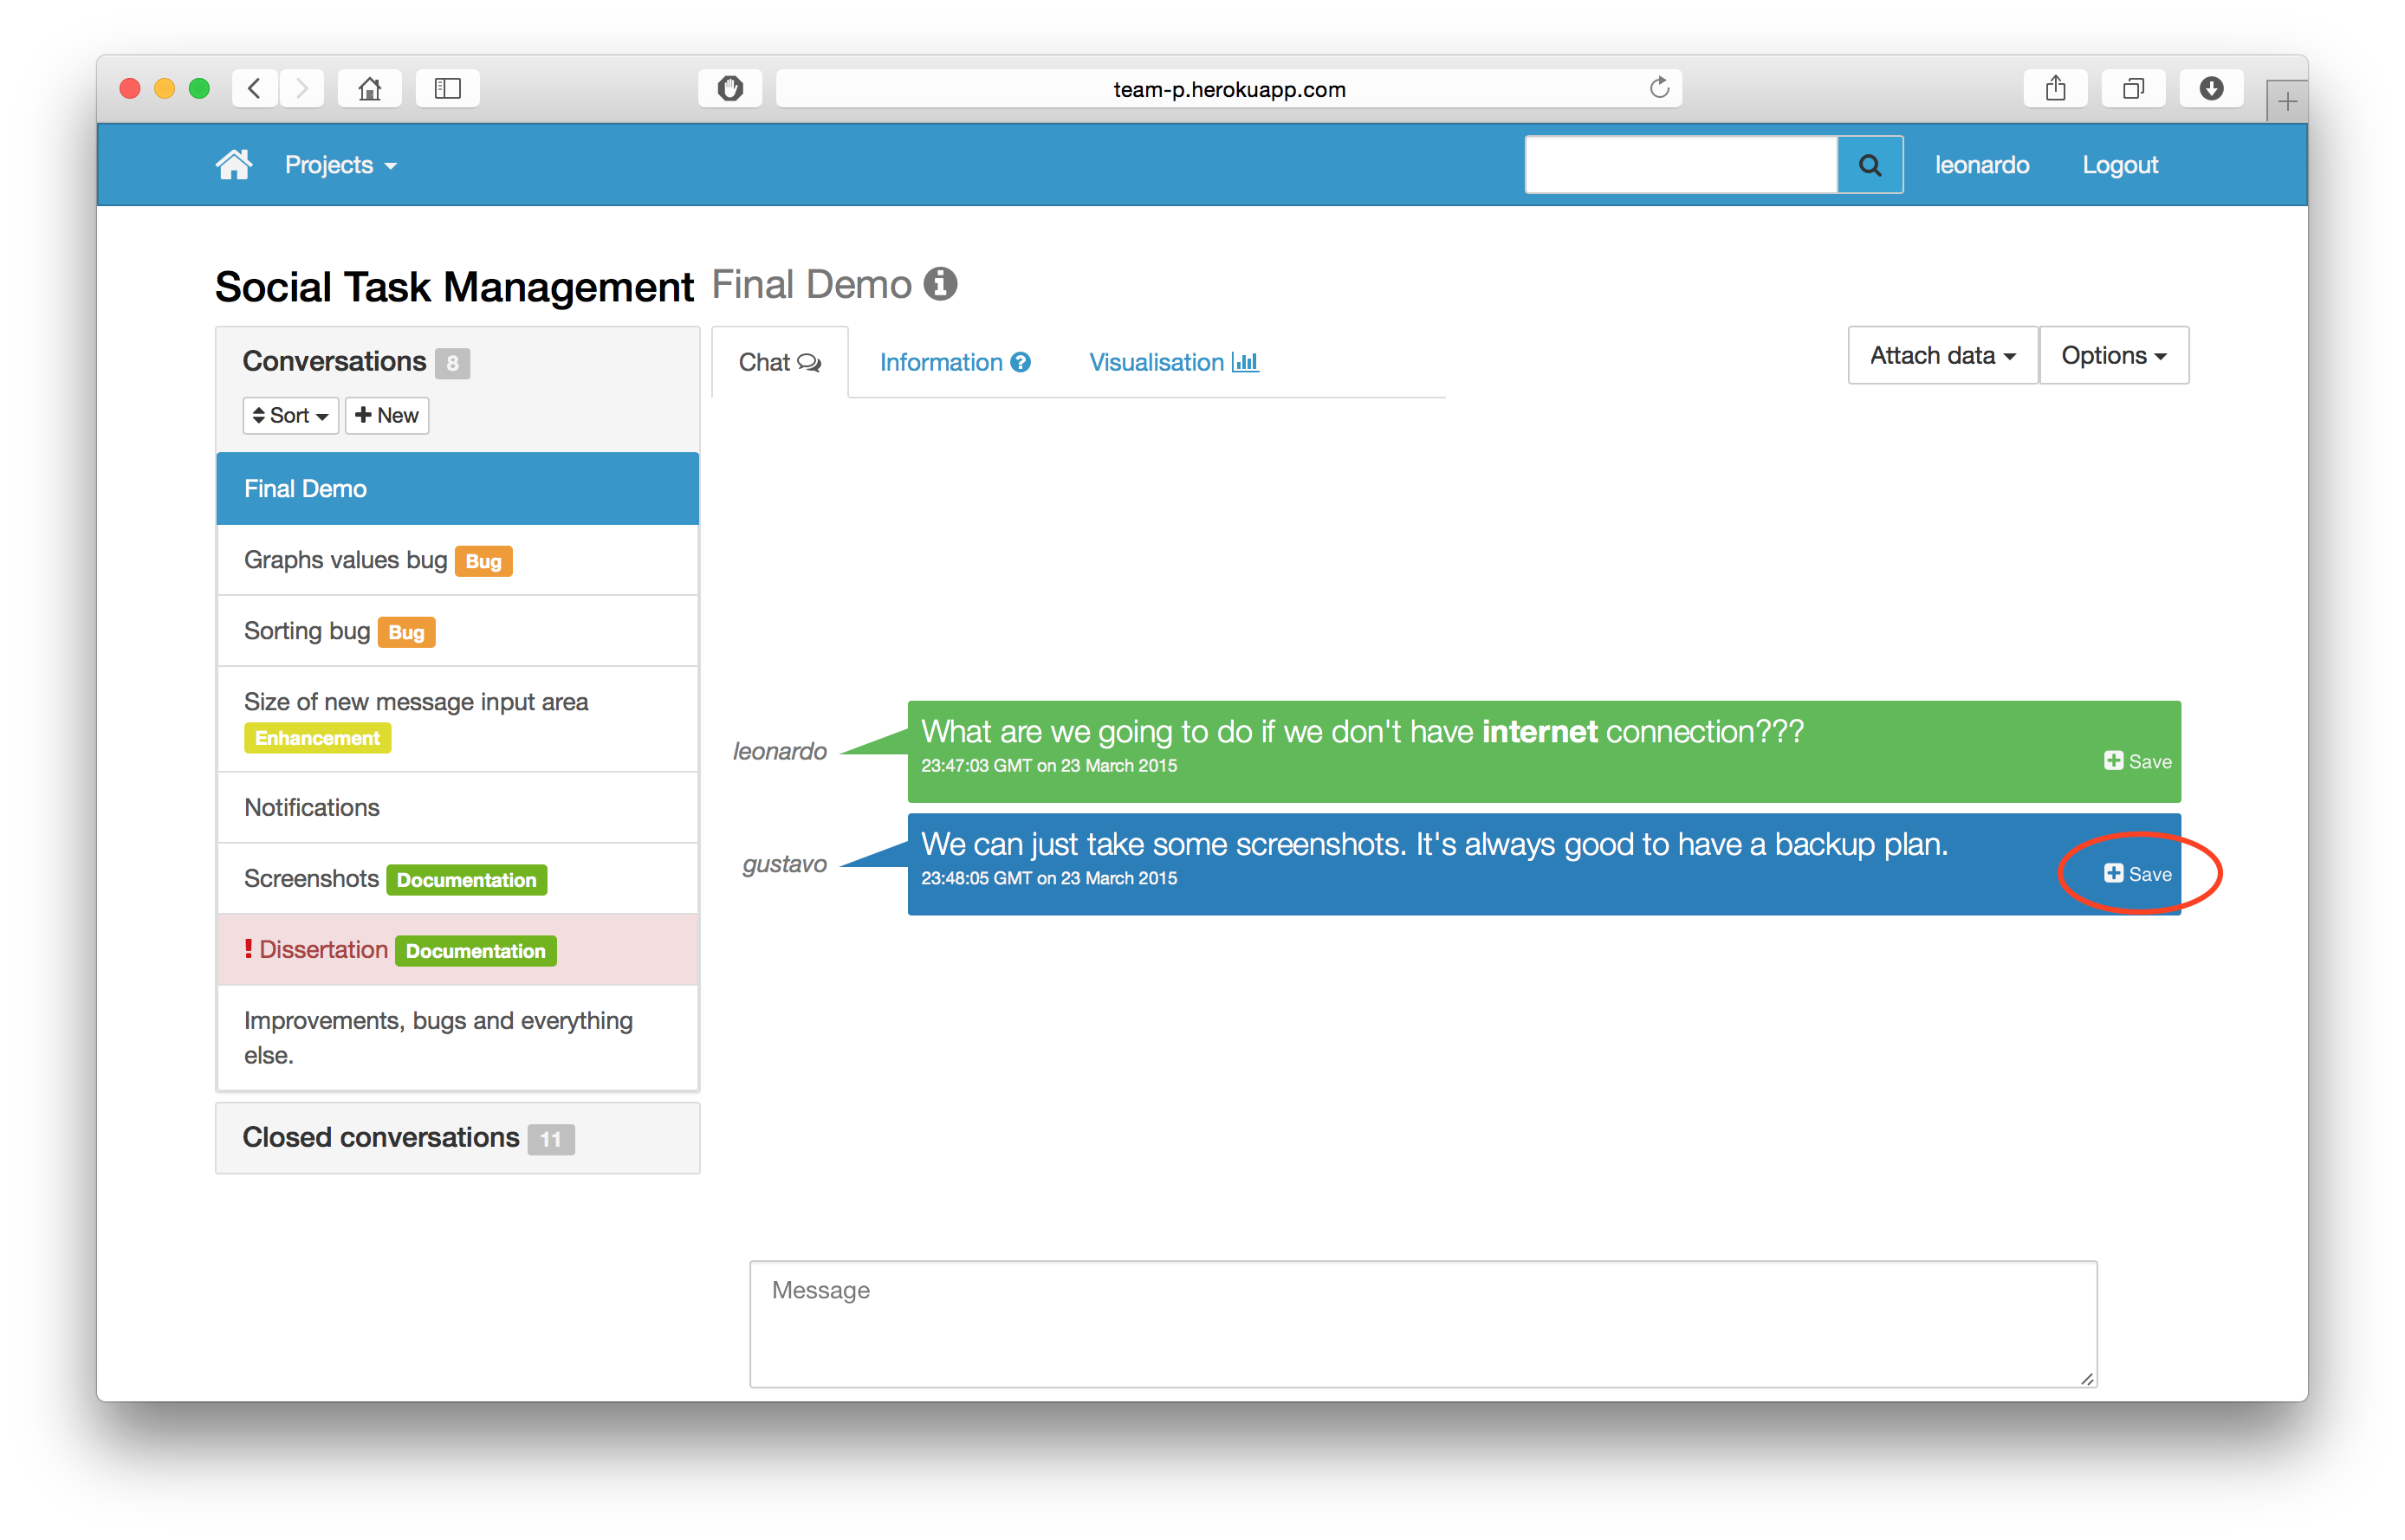
\includegraphics[width=\textwidth]{saveMessage}
		\caption{Saving a message}
		\label{fig:saveMessage}        
    \end{subfigure}
    \begin{subfigure}[b]{0.48\textwidth}
        \centering
		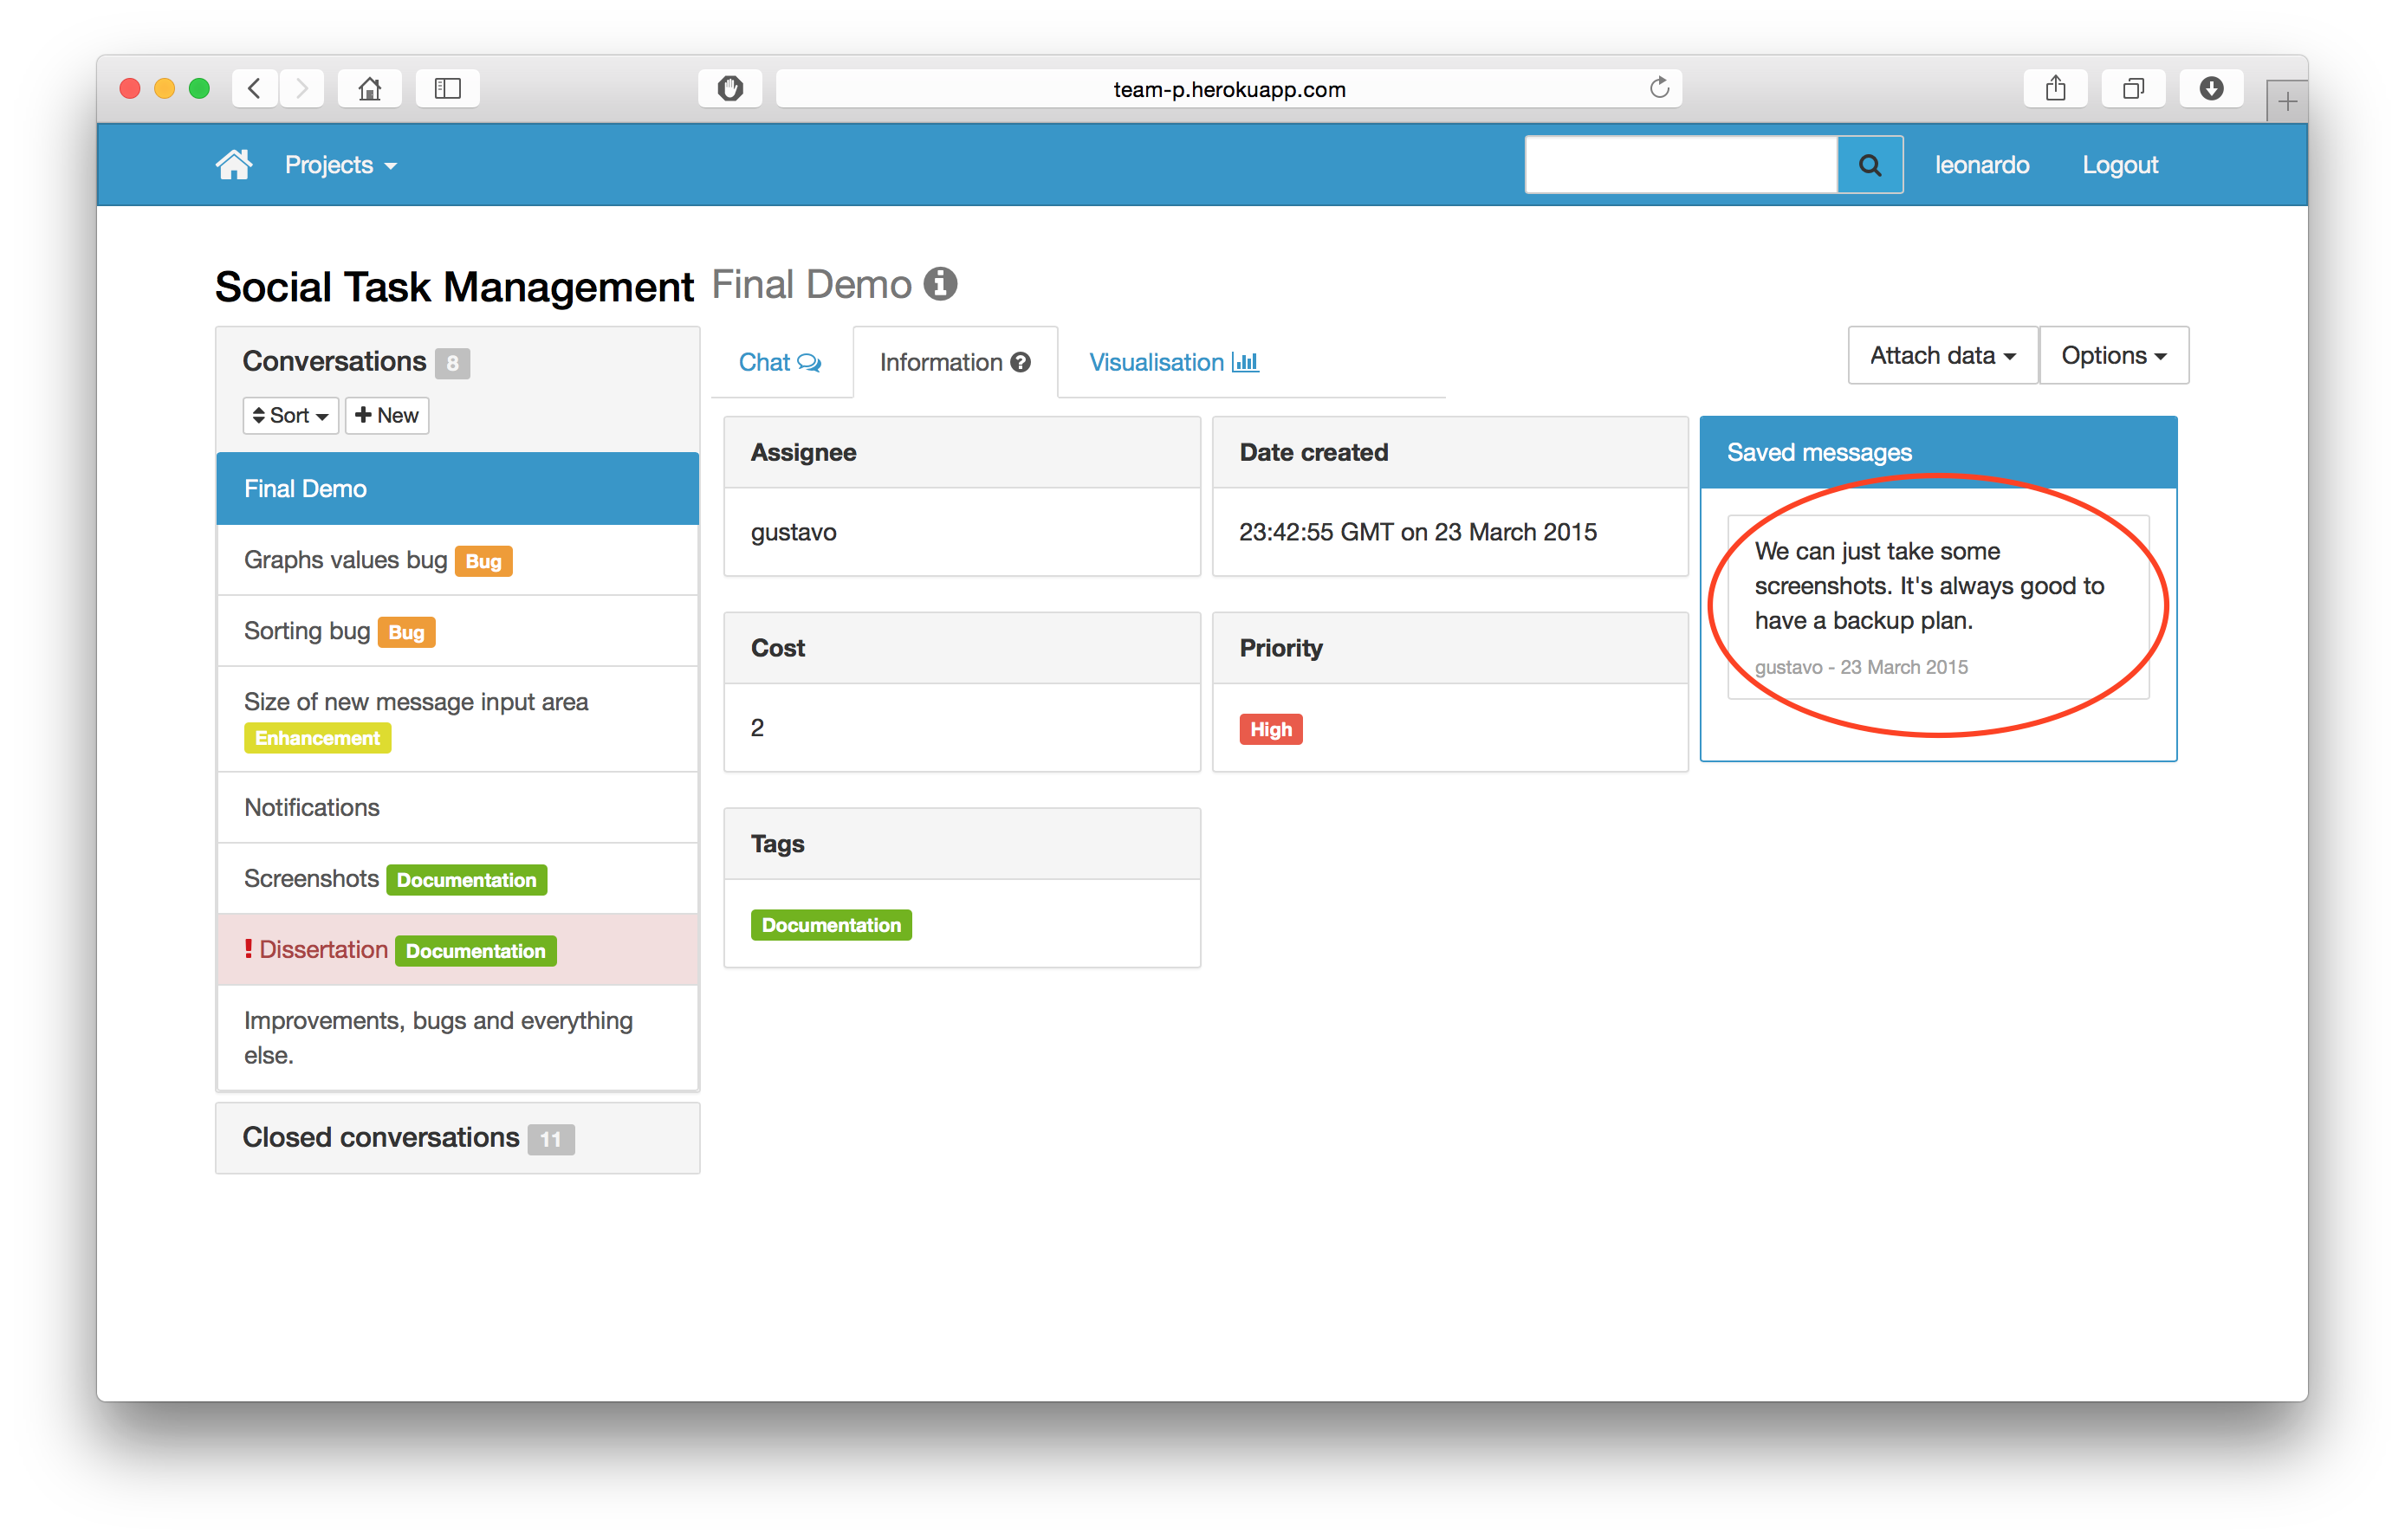
\includegraphics[width=\textwidth]{messageSaved}
		\caption{Message saved}
		\label{fig:messageSaved} 
    \end{subfigure}    
    \caption{Saved Messages feature}
    \label{fig:feature}
\end{figure}

With this feature, the user can have a list of all the relevant information in a chat and there is no need to read the entire conversation to understand what is happening. Thereby, there is no duplication of effort and every relevant content can be saved as the conversation is occurring.

\subsection{Improved Navigation}
\label{improved}

In extremely active projects, there can be many conversations in existence at any given time. Without any navigational assistance, finding a conversation could be cumbersome, even if the name of the conversation was known. 

To assist the user in finding what they need, filtering and sorting functionality was added. The user can sort conversations based on selected types of metadata such as due date and priority. As a result, conversations of particular interest can be identified with ease. 

Additionally, the user can filter the conversations based on their names. As the user types a string into the search input box, only conversations whose names contain this string as a substring will remain on screen, and the rest will be immediately hidden from view.

%============================================================================
\chapter{Evaluation}
\label{evaluation}

The project was formulated with the intent to create a ticket management system which emphasised communication between developers over coordination of data on a ticket. The resultant product does this effectively, by providing a means of associating additional information with a conversation. The name of a conversation equates to a ticket name, and the data that would be stored in a ticket using a conventional ticketing system is contained within the information tab of the chat.  This means that despite appearing at a glance like a primarily chat system, with metadata almost an afterthought, it provides the full functionality of a ticketing system.  

Due to this, the system can be used as a self contained system for project management, without need of external systems to ‘fill in the gaps’.

%----------------------------------------------------------------------------
\section{External Evaluation}
\label{externalEvaluation}

The team enlisted the help of another project team in evaluating the application.  From this a number of areas where the system performed well was ascertained, as well as areas of potential improvement.

It was found that the testers liked the overall layout, and believed the graphs could be helpful in exposing useful information about a project.  

However, a number of possible changes that were identified included:
\begin{itemize}
\item Metadata added was anonymous and thus open to abuse - it does not say who saves messages, who adds notes, etc.  Who added what should be shown in the information tab.
\item System is open to attacks to due major security issues.  API is not secure in that users can view and modify database objects through it.
\item An inclusion of a list of recent activity could greatly improve the usability of the site, allowing users to see what has been recently done on each project.

\item Allowing the user to customise the appearance, such as choosing a colour scheme or changing the font allows them to personalise it as they prefer and adds a sense of identity for different users.
\end{itemize}

%----------------------------------------------------------------------------
\section{Dogfooding}
\label{dogfooding}

As a result of the team using the application to manage their own project, they were able to evaluate the effectiveness of the tool.  As discussed in the previous section, the identification of key weaknesses allowed the team to fix these and improve the user experience as a whole.  As the team are part of the target market they were in the optimal position to evaluate the usefulness of the system as a whole, and with the inclusion of the additional features it was found that the tool functions as a wholly inclusive management system, while remaining easy to use.

Some key additions were made to the functionality of the application as a result of the team experiencing it as users. For example, the need for a saved messages functionality was quickly identified and its inclusion proved very useful. Also, notifications were added after this part of the project’s evaluation. It became evident that the messaging system suffered from a lacking of updating users on activity, meaning that issues could go untreated as no developers were aware of new information. 
%----------------------------------------------------------------------------
\section{Future Goals}
\label{futureGoals}

\subsection{Security and Stability}
\label{security}
As noted in the external evaluation section, the API remains public and so if someone can access the server that the application is deployed on, they will gain limited access to the REST API for that deployment instance. Therefore, checking whether the request is from an authenticated source is a high priority goal for the future. Additionally, using the “security rules” feature provided by Firebase, conversations can be made more secure by ensuring only users participating in a conversation and managers can see the messages within.

In order to improve the robustness of the application, the user interface could be tested using a tool such as Selenium WebDriver. Selenium \cite{site:selenium} automates web browsers by automatically performing user defined actions to ensure that web applications are working as expected.

\subsection{Update Feed}
\label{updating}
The landing page of the application is currently lacking in content and could be updated in order to provide a “birds-eye” view of all things happening within the user’s projects. Displaying a feed summarising all of the latest messages, conversations and high priority issues would vastly improve the capabilities of the software as project management suite. Managers would no longer have to check individual conversations or rely solely on the provided metrics, but could also receive up to the minute updates on the latest happenings within their projects. A feature like this would be particularly helpful in large scale software projects, where it would be infeasible to manually check each conversation for progress updates.

Additionally, mobile users currently do not receive notifications, but users are frequently away from their keyboards and may need to be aware of an issue immediately. Native mobile applications would provide a richer mobile experience, and would also be capable of delivering notifications straight to a user’s smartphone or tablet. 

\subsection{Integrating with Third Parties}
\label{integration}
Feedback received as a result of the prototype demonstration in December suggested that integration with a service such as Jenkins may be a valuable addition to the application. Jenkins \cite{site:jenkins}is a continuous integration server used to monitor and execute repeated jobs, such as building and testing software being developed.  This could be implemented through treating Jenkins as a user who would automatically create a ticket based on each build.  It could also automatically create a high priority ticket when a build fails, and tag the relevant developers.  Jenkins provides a REST API, which would make this integration relatively simple.

Another potential addition could be integration with Github or version control systems such as Subversion. Version control systems often allow for issues to be noted within commits, and discussing these issues as tickets within this application would be useful.  For example, a conversation could be created automatically when a pull request (a request to merge one branch into another) is created on Github.  This could be used to discuss the changes being made and suggest possible modifications.

\subsection{Scalability}
\label{scalability}

Currently, the setup of the project is such that it may not easily scale to large software development teams of hundreds or thousands of developers. 
One solution to this problem would be to filter conversations only be those a user has interacted with. To add another developer to a conversation, a user may “tag” the other developer using a notation such as “@username”. This would allow for a user to easily see the conversations that concern them, but would come at the cost of the user’s awareness of the project at large, as to list all conversations within an excessively large project would take an enormous amount of screen space. 

A second solution to this problem would be to allow for sub-projects. This would permit work to be broken into smaller chunks (an instance of the application managing a game could include a game engine project, with a game physics sub-project). This would require some alterations to the user interface, but would allow for effective management of projects in a way that is currently difficult with many popular project management tools such as Trac. Additionally, this would work well with the previously suggested feed of recent content, as users could see recent content in the context of its more specific sub-project title, rather than the context of an all-encompassing project title. 



%============================================================================
\chapter{Conclusion}
\label{conclusion}

As shown by the team’s self evaluation of the application, the project is currently in a stable and useful enough state that it can be used to monitor and track issues within a software development team. 

The final project serves well as an example of how project management can benefit from a focus on communication in a ticket management scenario. In integrating communication and ticket management, it has been found through the team’s own usage of the application that communication is a vital component of a ticket’s lifecycle. Furthermore, the application shows that ticket management can benefit from an increased focus on communication over what currently used products provide. The project has achieved its aims of providing a ticket management system which treats an ordinary conversation as a ticket, and is a viable enough solution to be useful for at least small software development teams. 

While some problems persist in the project, as exposed in the external evaluation, the utility of the project was evident to those who viewed it. This shows that there is a definite lacking in the integration of ticket management and instant messaging within project management. It also shows that communication between developers is unnecessarily complicated by current tools. 

%============================================================================
\bibliography{dissertation}{}
\bibliographystyle{acm}

\end{document}
